\documentclass[11pt]{article}

% Change "review" to "final" to generate the final (sometimes called camera-ready) version.
\usepackage[review]{acl}

% Standard package includes
\usepackage{times}
\usepackage{latexsym}
\usepackage[T1]{fontenc}
\usepackage[utf8]{inputenc}
\usepackage{microtype}
\usepackage{graphicx}
\usepackage{amsmath}
\usepackage{amssymb}
\usepackage{booktabs}
\usepackage{multirow}
\usepackage{xcolor}
\usepackage{subcaption}
\usepackage{tikz}
\usepackage{pgfplots}
\pgfplotsset{compat=1.17}
\usetikzlibrary{positioning,arrows.meta,shapes.geometric,fit,backgrounds,patterns}

% Custom commands
\newcommand{\method}{VGA-Fusion}
\newcommand{\vad}{VAD}

\title{Sentimentogram: Interpretable Multimodal Speech Emotion Recognition \\ with VAD-Guided Attention and Emotion-Aware Typography Visualization}

% Anonymous for review
%\author{Anonymous ACL submission}
\author{Mukhiddin Toshpulatov \\
	Voice AI Research Institute, Inha University \\
	Computer Science and Programming Dep. \\
	Jizzakh branch of National University of Uzb. \\
	259 Sh Rashidov, Jizzakh, Uzbekistan \\
	\texttt{muhiddin@inha.ac.kr} \\\And
	Seungkyu Oh \\
	Department of Industrial Engineering \\
	Inha University 100 Inha-ro, \\
	Michuhol-gu, Incheon 22212, Korea \\
	\texttt{december\_i@inha.edu} \\\AND
	Ulugbek Amankulov \\
	Munhak Information High School \\
	350 Soseong-ro, Michuhol-gu \\
	Incheon 22212, Korea \\
	\texttt{ulugbekamankulov13pro@gmail.com} \\\And
	Suan Lee \\
	School of Computer Science \\
	Semyung University \\
	65 Semyung-ro, Jecheon 27136, Korea \\
	\texttt{suanlee@semyung.ac.kr} \\\AND
	Kuvandikov Jo'ra Tursunbayevich \\
	Computer Science and Programming Dep. \\
	Jizzakh branch of National University of Uzb. \\
	259 Sh Rashidov, Jizzakh, Uzbekistan \\
	\texttt{jorakuvandikov1@gmail.com} \\\And
	Gadaev Doniyor \\
	Faculty of Pedagogy and Psychology \\
	Jizzakh state pedagogical university \\
	4 Rashidov, 130100, Jizzakh, Uzbekistan \\
	\texttt{muxiddin1979@gmail.com} \\\AND
	Wookey Lee \\
	Department of Industrial and \\
	Biomedical Science Engineering \\
	Inha University 100 Inha-ro, \\
	Michuhol-gu, Incheon 22212, Korea \\
	\texttt{trinity@inha.ac.kr} \\}
  
\begin{document}
\maketitle

%==============================================================================
% ABSTRACT
%==============================================================================
\begin{abstract}
We present \textbf{Sentimentogram}, a \textit{human-centered} framework that bridges the gap between speech emotion recognition (SER) models and human understanding. Unlike prior work focused solely on classification accuracy, our framework prioritizes three pillars: \textbf{interpretability}, \textbf{visualization}, and \textbf{personalization}. We contribute: (1) \textbf{Constrained Adaptive Fusion} with gates summing to one, enabling transparent per-sample modality contribution analysis (e.g., ``76\% audio, 24\% text''); (2) \textbf{VAD-Guided Cross-Attention} grounded in dimensional emotion psychology; (3) \textbf{Emotion-Aware Typography Visualization}---a novel system that renders word-level emotion predictions through dynamic fonts, colors, and sizes, transforming model outputs into human-readable subtitles; and (4) \textbf{Preference-Learning Personalization}---learning individual visualization preferences from pairwise comparisons, significantly outperforming rule-based cultural adaptation (+14.6\%, $p<0.05$). Crucially, we demonstrate that demographic-based style rules perform \textit{worse than random} (43.8\% vs 50.3\%), advocating for learned personalization in NLP interfaces. Our framework achieves competitive SER performance (IEMOCAP 5-class: 77.97\% UA) while providing the interpretability and user-centric design essential for real-world deployment. Demo video showcasing TED talk emotion typography available.\footnote{\url{https://drive.google.com/file/d/1jCQJbIAbtNDGf2GunXnjgWqmZWq9kvY6/view}} Code: \url{https://anonymous.4open.science/r/multimodal-ser}.
\end{abstract}

%==============================================================================
% INTRODUCTION
%==============================================================================
\section{Introduction}

The gap between machine learning models and human understanding represents a critical challenge for deploying emotion recognition systems in real-world applications. While speech emotion recognition (SER) has achieved impressive accuracy gains, end users cannot interpret model decisions, visualize predictions intuitively, or customize outputs to their preferences. We argue that \textit{human-centered design}---not just accuracy improvements---is essential for SER adoption in applications like mental health monitoring, accessibility tools, and media annotation.

Consider a therapist using SER for patient session analysis: they need to understand \textit{why} the model predicted anger (audio tone vs. word choice?), \textit{see} the emotion flow across the conversation, and \textit{personalize} how emotions are displayed based on their workflow. Current systems provide none of these capabilities.

We present \textbf{Sentimentogram}, a human-centered SER framework built on three pillars:

\paragraph{(1) Interpretable fusion.} We introduce \textbf{Constrained Adaptive Fusion} where modality gates sum to one, enabling direct interpretation: ``This prediction relied 76\% on audio, 24\% on text.'' Unlike black-box fusion, users can understand and trust model decisions.

\paragraph{(2) Emotion visualization.} Our \textbf{Emotion-Aware Typography} system transforms predictions into dynamic subtitles where each word's font, color, and size reflect its predicted emotion. This bridges the gap between model outputs and human perception.

\paragraph{(3) Learned personalization.} Rather than assuming preferences from demographics (which we show performs \textit{worse than random}), our \textbf{Preference-Learning} module learns individual visualization preferences from minimal pairwise feedback (+14.6\% over rule-based, $p<0.05$).

Additionally, we contribute \textbf{VAD-Guided Cross-Attention} grounded in dimensional emotion theory \citep{russell1980circumplex}, and \textbf{Hard Negative Mining MICL} for robust cross-modal alignment.

Our framework achieves competitive SER performance (IEMOCAP 5-class: 77.97\% UA; CREMA-D: 92.90\% UA) while providing the interpretability, visualization, and personalization essential for deployment. Our contributions are:

\begin{itemize}
    \item \textbf{Interpretable Fusion} (Section~\ref{sec:fusion}): Constrained gates with sum-to-one constraint for transparent modality contribution analysis---the first fusion mechanism enabling per-sample explanations.

    \item \textbf{Emotion-Aware Typography} (Section~\ref{sec:visualization}): A novel real-time visualization system transforming SER predictions into dynamic subtitles with emotion-specific fonts, colors, and sizes.

    \item \textbf{Preference-Learning Personalization} (Section~\ref{sec:personalization}): Data-driven style adaptation that learns from pairwise comparisons, demonstrating that rule-based cultural assumptions fail while learned models succeed.

    \item \textbf{VAD-Guided Attention} (Section~\ref{sec:vga}): Psychology-grounded cross-attention incorporating Valence-Arousal-Dominance theory.

    \item \textbf{Human-Centered Evaluation}: Beyond accuracy metrics, we evaluate interpretability through fusion gate analysis and personalization through user preference prediction.

    \item \textbf{Preference Dataset}: We release the first visualization preference dataset for emotion-aware typography, enabling future research in personalized NLP interfaces.
\end{itemize}

These three pillars form a cohesive pipeline: \textbf{interpretable fusion} enables users to understand \textit{why} the model made a prediction (e.g., ``audio dominated because the speaker's tone was aggressive''); \textbf{visualization} transforms this understanding into \textit{what} users see (emotion-styled subtitles); and \textbf{personalization} determines \textit{how} users prefer to see it (learned style preferences). This integration is crucial---interpretability without visualization remains inaccessible to end-users, and visualization without personalization assumes one-size-fits-all preferences.

We position Sentimentogram as a step toward \textit{explainable and user-centric NLP systems}, where model decisions are transparent, outputs are human-readable, and interfaces adapt to individual users.

\paragraph{Distinction from prior fusion work.} While cross-attention mechanisms are well-established \citep{tsai2019multimodal}, our contribution is \textit{not} another fusion architecture for accuracy gains. Instead, we contribute: (1) \textit{interpretability} through constrained gates (existing methods are black-box); (2) \textit{visualization} that transforms predictions into human-readable outputs (no prior SER work does this); and (3) \textit{personalization} through preference learning (demonstrating rule-based approaches fail). The fusion mechanism is a means to an end---enabling the human-centered pipeline that is our primary contribution.

%==============================================================================
% RELATED WORK
%==============================================================================
\section{Related Work}

\subsection{Unimodal Speech Emotion Recognition}

Traditional SER relied on handcrafted acoustic features like MFCCs and prosodic measures \citep{schuller2018speech}. The transformer architecture \citep{vaswani2017attention} has revolutionized this field. Self-supervised models have achieved significant progress: wav2vec2 \citep{baevski2020wav2vec} learns general speech representations, HuBERT \citep{hsu2021hubert} uses masked prediction for speech modeling, WavLM \citep{chen2022wavlm} enables full-stack speech processing, and emotion2vec \citep{ma2024emotion2vec} specifically targets emotion-discriminative features. Recent work has explored speaker normalization \citep{gat2022speaker}, temporal modeling \citep{ye2023temporal}, and combining supervised with self-supervised learning \citep{chen2023exploring}. Wagner et al. \citep{wagner2023dawn} provide a comprehensive analysis of transformer-based SER, highlighting the persistent valence gap challenge.

\subsection{Multimodal Fusion for SER}

Early multimodal approaches used simple concatenation or late fusion \citep{poria2017review}. The Multimodal Transformer (MulT) introduced crossmodal attention for unaligned sequences \citep{tsai2019multimodal, safarov2025hyperspectral}, achieving 74.1\% on IEMOCAP. MISA \citep{hazarika2020misa} learned modality-invariant and modality-specific representations with adversarial training, reaching 76.4\%. MMIM \citep{han2021improving} applied mutual information maximization for fusion, obtaining 77.0\%. Attention bottlenecks \citep{nagrani2021attention} have been explored for efficient multimodal fusion.

Recent work has explored knowledge distillation \citep{chudasama2022telme}, universal frameworks for cross-corpus SER \citep{pepino2023uniser}, and multimodal visualization \citep{liang2023multiviz}. Cross-modal contrastive learning approaches \citep{yu2023connecting} have shown promise for alignment. However, these methods lack interpretability---they do not reveal how modalities contribute to predictions.

\subsection{Dimensional Emotion Models}

The VAD model \citep{russell1980circumplex} represents emotions along three dimensions: Valence (positive/negative), Arousal (activation level), and Dominance (control). While VAD annotations exist for emotion lexicons \citep{mohammad2018obtaining}, no prior work has used VAD to guide cross-modal attention mechanisms.

\subsection{Contrastive Learning for Multimodal Alignment}

CLIP \citep{radford2021learning} demonstrated the power of contrastive learning for vision-language alignment. SimCLR \citep{chen2020simple} established the framework for visual contrastive learning, while SimCSE \citep{gao2021simcse} adapted it for sentence embeddings. In multimodal sentiment, contrastive objectives have improved representation learning \citep{mai2022hybrid}. Recent work has explored contrastive language-audio pretraining \citep{wang2024clap} and semi-supervised multimodal learning \citep{lian2024smin}. However, standard approaches use random negatives, which may be suboptimal for emotion recognition where some emotions are easily distinguishable.

\subsection{Recent Advances in Multimodal SER}

Recent work incorporates LLMs into multimodal SER: MPLMM \citep{guo2024mplmm} handles missing modalities, EmoBox \citep{ma2024emobox} establishes multilingual benchmarks, and EmoLLM \citep{chen2024emollm} enables multimodal emotional understanding. InstructERC \citep{li2024instructerc} and DialogueLLM \citep{zou2024dialoguellm} leverage conversational context. For utterance-level methods, speaker-aware approaches like SDIF \citep{wang2024sdif} and conversational models (DAG-ERC \citep{shen2021directed}, EmoCaps \citep{li2022emocaps}) have advanced the field.

\subsection{Emotion Visualization in NLP}

Prior work on sentiment/emotion visualization has focused primarily on document-level or sentence-level representations \citep{kucher2018text}. Sentiment word clouds, color-coded highlights, and timeline charts are common approaches. Related works in facial animation and talking face generation \citep{toshpulatov2021generative, toshpulatov2023talking} have explored visual emotion rendering, while human body language understanding \citep{toshpulatov2022human,toshpulatov2024ddc3n, toshpulatov2025deep} provide complementary non-verbal cues. However, \textbf{word-level emotion typography}---where font family, size, spacing, and animation dynamically reflect predicted emotions---remains unexplored. Our Sentimentogram fills this gap with culturally-adapted (Western/Eastern) real-time visualization.

\subsection{Preference Learning and Personalization}

Preference learning from pairwise comparisons has been studied extensively \citep{thurstone1927law,bradley1952rank, bae2023diffusion}. Recent work applies preference learning to recommendation systems \citep{koren2009matrix}, language model alignment \citep{christiano2017deep,ouyang2022training}, and personalized text generation \citep{li2016persona}. In HCI, personalization of visual interfaces has explored adaptive layouts \citep{findlater2004comparison} and accessibility features \citep{bigham2017making}. However, \textbf{personalized emotion visualization}---learning individual preferences for how emotions should be displayed---remains unexplored. Our preference learning approach addresses this gap, showing that learned personalization significantly outperforms fixed cultural rules.

%==============================================================================
% METHOD
%==============================================================================
\section{Method}

Figure~\ref{fig:architecture} illustrates our \method{} architecture. Given text features from BERT and audio features from emotion2vec, we project them to a shared space, apply VAD-guided cross-attention, fuse with constrained adaptive fusion, and classify with focal loss.

\begin{figure*}[!t]
\centering
\resizebox{0.85\textwidth}{!}{%
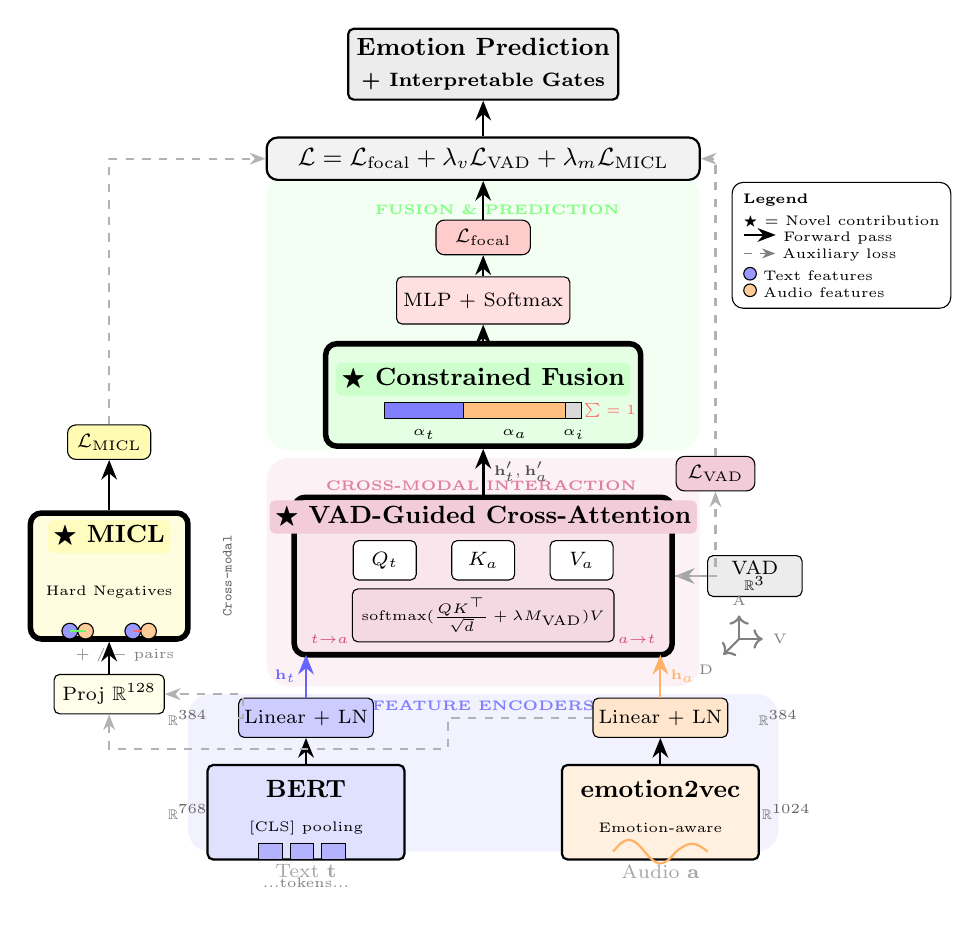
\begin{tikzpicture}[
    % Modern scholarly styles inspired by MulT/MISA/CLIP/Transformer papers
    encoder/.style={draw, thick, rounded corners=2pt, minimum width=2.2cm, minimum height=1.2cm, align=center, font=\small\bfseries, inner sep=3pt},
    module/.style={draw, line width=1.2pt, rounded corners=4pt, minimum height=1.1cm, align=center, font=\small\bfseries, inner sep=4pt},
    submodule/.style={draw, rounded corners=2pt, minimum width=1.4cm, minimum height=0.5cm, align=center, font=\scriptsize, inner sep=2pt},
    tensor/.style={draw, fill=white, minimum width=0.4cm, minimum height=0.8cm, font=\tiny},
    arrow/.style={-{Stealth[length=2.5mm, width=2mm]}, thick},
    dasharrow/.style={-{Stealth[length=2mm]}, thick, dashed, gray!60},
    tensorarrow/.style={-{Stealth[length=2mm]}, thick, blue!60},
    labelstyle/.style={font=\scriptsize, text=gray!70},
    dimstyle/.style={font=\tiny\ttfamily, text=black!60},
    groupbox/.style={draw, dashed, rounded corners=6pt, inner sep=8pt, gray!40}
]

% ============ BACKGROUND GROUPS ============
\begin{scope}[on background layer]
    % Input encoders group - minimal padding
    \fill[blue!5, rounded corners=8pt] (-1.5,0.0) rectangle (6.0,2.0);
    \node[font=\tiny\bfseries, text=blue!50] at (2.25,1.85) {FEATURE ENCODERS};

    % Cross-modal interaction group - adjusted for moved modules
    \fill[purple!5, rounded corners=8pt] (-0.5,2.1) rectangle (5.0,5.0);
    \node[font=\tiny\bfseries, text=purple!50] at (2.225,4.645) {CROSS-MODAL INTERACTION};

    % Fusion & prediction group
    \fill[green!5, rounded corners=8pt] (-0.5,5.1) rectangle (5.0,8.6);
    \node[font=\tiny\bfseries, text=green!50] at (2.43,8.15) {FUSION \& PREDICTION};
\end{scope}

% ============ INPUT REPRESENTATIONS ============
% Text encoder with internal structure
\node[encoder, fill=blue!12, minimum width=2.5cm] (bert) at (0,0.5) {};
\node[font=\small\bfseries] at (0,0.8) {BERT};
\node[font=\tiny] at (0,0.3) {[CLS] pooling};
\draw[fill=blue!30] (-0.6,-0.1) rectangle (-0.3,0.1);
\draw[fill=blue!30] (-0.2,-0.1) rectangle (0.1,0.1);
\draw[fill=blue!30] (0.2,-0.1) rectangle (0.5,0.1);
\node[font=\tiny, text=gray] at (0,-0.4) {...tokens...};

% Audio encoder with internal structure
\node[encoder, fill=orange!12, minimum width=2.5cm] (e2v) at (4.5,0.5) {};
\node[font=\small\bfseries] at (4.5,0.8) {emotion2vec};
\node[font=\tiny] at (4.5,0.3) {Emotion-aware};
% Waveform visualization
\draw[orange!60, thick] (3.9,0) sin (4.1,0.15) cos (4.3,0) sin (4.5,-0.15) cos (4.7,0) sin (4.9,0.1) cos (5.1,0);

% Dimension annotations
\node[dimstyle] at (-1.5,0.5) {$\mathbb{R}^{768}$};
\node[dimstyle] at (6.1,0.5) {$\mathbb{R}^{1024}$};

% Input labels - integrated with encoders
\node[labelstyle] at (0,-0.25) {Text $\mathbf{t}$};
\node[labelstyle] at (4.5,-0.25) {Audio $\mathbf{a}$};

% ============ PROJECTION LAYERS ============
\node[submodule, fill=blue!20] (proj_t) at (0,1.7) {Linear + LN};
\node[submodule, fill=orange!20] (proj_a) at (4.5,1.7) {Linear + LN};
\node[dimstyle] at (-1.5,1.7) {$\mathbb{R}^{384}$};
\node[dimstyle] at (6.0,1.7) {$\mathbb{R}^{384}$};

\draw[arrow] (bert) -- (proj_t);
\draw[arrow] (e2v) -- (proj_a);

% ============ VAD-GUIDED CROSS-ATTENTION (Novel 1) ============
% Main VGA module with detailed internal structure - moved down more for clear visibility
\node[module, fill=purple!10, minimum width=4.8cm, minimum height=2.0cm, line width=2pt] (vga_main) at (2.25,3.5) {};

% VGA title with star - positioned inside module, above internal blocks
\node[font=\small\bfseries, fill=purple!20, rounded corners=2pt, inner sep=2pt] at (2.25,4.25) {$\bigstar$ VAD-Guided Cross-Attention};

% Internal attention structure
\node[submodule, fill=white, minimum width=0.8cm] (q1) at (1.0,3.7) {$Q_t$};
\node[submodule, fill=white, minimum width=0.8cm] (k1) at (2.25,3.7) {$K_a$};
\node[submodule, fill=white, minimum width=0.8cm] (v1) at (3.5,3.7) {$V_a$};

% Attention computation box
\node[draw, fill=purple!15, rounded corners=2pt, minimum width=2.8cm, minimum height=0.5cm, font=\tiny] (attn) at (2.25,3.0) {$\text{softmax}(\frac{QK^\top}{\sqrt{d}} + \lambda M_{\text{VAD}})V$};

% VAD projection with 3D indicator
\node[submodule, fill=gray!15, minimum width=1.2cm] (vad) at (5.7,3.5) {VAD\\[-2pt]\tiny$\mathbb{R}^3$};
% 3D VAD space visualization
\draw[->, gray, thick] (5.5,2.7) -- (5.8,2.7) node[right, font=\tiny] {V};
\draw[->, gray, thick] (5.5,2.7) -- (5.5,3.0) node[above, font=\tiny] {A};
\draw[->, gray, thick] (5.5,2.7) -- (5.3,2.5) node[below left, font=\tiny] {D};

% Bidirectional arrows annotation
\node[font=\tiny, text=purple!70] at (0.3,2.7) {$t{\rightarrow}a$};
\node[font=\tiny, text=purple!70] at (4.2,2.7) {$a{\rightarrow}t$};

% Input arrows to VGA module - straight vertical arrows from projections to module
\draw[arrow, thick, blue!60] (proj_t.north) -- (0,2.5) node[midway, left, font=\tiny, text=blue!60] {$\mathbf{h}_t$};
\draw[arrow, thick, orange!60] (proj_a.north) -- (4.5,2.5) node[midway, right, font=\tiny, text=orange!60] {$\mathbf{h}_a$};
\draw[arrow, gray!70] (vad) -- (vga_main.east);

% ============ MICL BRANCH (Novel 3) ============
\node[module, fill=yellow!12, minimum width=2.0cm, minimum height=1.6cm, line width=2pt] (micl_main) at (-2.5,3.5) {};
\node[font=\small\bfseries, fill=yellow!25, rounded corners=2pt, inner sep=2pt] at (-2.5,4.0) {$\bigstar$ MICL};
\node[font=\tiny] at (-2.5,3.3) {Hard Negatives};

% Contrastive visualization (positive/negative pairs)
\draw[fill=blue!40] (-3.0,2.8) circle (0.1);
\draw[fill=orange!40] (-2.8,2.8) circle (0.1);
\draw[green!60, thick] (-3.0,2.8) -- (-2.8,2.8);
\draw[fill=blue!40] (-2.2,2.8) circle (0.1);
\draw[fill=orange!40] (-2.0,2.8) circle (0.1);
\draw[red!60, thick, dashed] (-2.2,2.8) -- (-2.0,2.8);
\node[font=\tiny, text=gray] at (-2.3,2.5) {$+$ / $-$ pairs};

\node[submodule, fill=yellow!8] (micl_proj) at (-2.5,2.0) {Proj $\mathbb{R}^{128}$};

\draw[dasharrow] (proj_t.west) -- (-0.8,1.7) -- (-0.8,2.0) -- (micl_proj.east);
\draw[dasharrow] (proj_a.west) -- (1.8,1.7) -- (1.8,1.3) -- (-2.5,1.3) -- (micl_proj.south);
\draw[arrow] (micl_proj) -- (micl_main);

% ============ CONSTRAINED ADAPTIVE FUSION (Novel 2) ============
% Positioned with proper spacing above VGA module
\node[module, fill=green!10, minimum width=4.0cm, minimum height=1.3cm, line width=2pt] (fusion) at (2.25,5.8) {};
\node[font=\small\bfseries, fill=green!20, rounded corners=2pt, inner sep=2pt] at (2.25,6.0) {$\bigstar$ Constrained Fusion};

% Gate visualization as stacked bar
\draw[fill=blue!50] (1.0,5.5) rectangle (2.0,5.7);
\draw[fill=orange!50] (2.0,5.5) rectangle (3.3,5.7);
\draw[fill=gray!30] (3.3,5.5) rectangle (3.5,5.7);
\node[font=\tiny] at (1.5,5.3) {$\alpha_t$};
\node[font=\tiny] at (2.65,5.3) {$\alpha_a$};
\node[font=\tiny] at (3.4,5.3) {$\alpha_i$};
\node[font=\tiny, text=red!60] at (3.860,5.6) {$\sum=1$};

% Connection from VGA to Fusion - single clear arrow with label
\draw[arrow, very thick] (vga_main.north) -- node[right, font=\tiny, text=black!70] {$\mathbf{h}'_t, \mathbf{h}'_a$} (fusion.south);

% ============ CLASSIFICATION HEAD ============
\node[submodule, fill=red!12, minimum width=2.2cm, minimum height=0.6cm] (cls) at (2.25,7.0) {MLP + Softmax};
\draw[arrow] (fusion) -- (cls);

% ============ MULTI-TASK LOSSES ============
\node[draw, fill=red!20, rounded corners=3pt, minimum width=1.2cm, font=\scriptsize] (loss_cls) at (2.25,7.8) {$\mathcal{L}_{\text{focal}}$};
\node[draw, fill=purple!20, rounded corners=3pt, minimum width=1.0cm, font=\scriptsize] (loss_vad) at (5.2,4.8) {$\mathcal{L}_{\text{VAD}}$};
\node[draw, fill=yellow!30, rounded corners=3pt, minimum width=1.0cm, font=\scriptsize] (loss_micl) at (-2.5,5.2) {$\mathcal{L}_{\text{MICL}}$};

\draw[arrow] (cls) -- (loss_cls);
\draw[dasharrow] (vga_main.east) -- (5.2,3.5) -- (loss_vad.south);
\draw[arrow] (micl_main) -- (loss_micl);

% ============ TOTAL LOSS ============
\node[draw, thick, rounded corners=4pt, fill=gray!10, minimum width=5.5cm, font=\small, inner sep=4pt] (total) at (2.25,8.8) {$\mathcal{L} = \mathcal{L}_{\text{focal}} + \lambda_v\mathcal{L}_{\text{VAD}} + \lambda_m\mathcal{L}_{\text{MICL}}$};
\draw[arrow] (loss_cls) -- (total);
\draw[dasharrow] (loss_vad) |- (total.east);
\draw[dasharrow] (loss_micl) |- (total.west);

% ============ OUTPUT ============
\node[encoder, fill=gray!15, minimum width=3cm, minimum height=0.9cm] (output) at (2.25,10.0) {Emotion Prediction\\{\scriptsize + Interpretable Gates}};
\draw[arrow] (total) -- (output);

% ============ LEGEND ============
\node[draw, rounded corners=4pt, fill=white, align=left, font=\tiny, inner sep=4pt] at (6.8,7.7) {
\textbf{Legend}\\[2pt]
$\bigstar$ = Novel contribution\\
\tikz\draw[-{Stealth}, thick] (0,0) -- (0.4,0); Forward pass\\
\tikz\draw[-{Stealth}, dashed, gray] (0,0) -- (0.4,0); Auxiliary loss\\[2pt]
\tikz\draw[fill=blue!40] (0,0) circle (0.08); Text features\\
\tikz\draw[fill=orange!40] (0,0) circle (0.08); Audio features
};

% ============ TENSOR FLOW ANNOTATIONS ============
\node[dimstyle, rotate=90] at (-1.0,3.5) {Cross-modal};

\end{tikzpicture}
}
\caption{The \method{} architecture with three novel contributions ($\bigstar$). \textbf{(1) VAD-Guided Cross-Attention}: Bidirectional attention modulated by Valence-Arousal-Dominance affinity matrix $M_{\text{VAD}}$, grounded in dimensional emotion theory \citep{russell1980circumplex}. \textbf{(2) Constrained Adaptive Fusion}: Interpretable gates ($\alpha_t + \alpha_a + \alpha_i = 1$) reveal per-sample modality contributions. \textbf{(3) Hard Negative Mining MICL}: Cross-modal contrastive learning \citep{radford2021learning} with curriculum-based hard negative sampling. Multi-task training combines focal loss, VAD regression, and MICL. Architecture inspired by MulT \citep{tsai2019multimodal} and MISA \citep{hazarika2020misa}.}
\label{fig:architecture}
\end{figure*}

\subsection{Feature Extraction}

We extract text features using BERT-base \citep{devlin2019bert}, taking the [CLS] token representation $\mathbf{t} \in \mathbb{R}^{768}$. For audio, we use emotion2vec-plus-large \citep{ma2024emotion2vec}, obtaining utterance-level embeddings $\mathbf{a} \in \mathbb{R}^{1024}$. Both are projected to a common dimension $d=384$:
\begin{align}
    \mathbf{h}_t &= \text{LayerNorm}(\text{GELU}(W_t \mathbf{t} + b_t)) \\
    \mathbf{h}_a &= \text{LayerNorm}(\text{GELU}(W_a \mathbf{a} + b_a))
\end{align}

\subsection{VAD-Guided Cross-Attention}
\label{sec:vga}

Standard multi-head cross-attention computes:
\begin{equation}
    \text{Attn}(Q, K, V) = \text{softmax}\left(\frac{QK^\top}{\sqrt{d_k}}\right)V
\end{equation}

We introduce VAD-guided attention by projecting features to the VAD space and computing affinity based on VAD similarity:
\begin{align}
    \mathbf{v}_t &= W_{\text{VAD}} \mathbf{h}_t, \quad \mathbf{v}_a = W_{\text{VAD}} \mathbf{h}_a \\
    M_{\text{VAD}}(i,j) &= -\|\mathbf{v}_t^{(i)} - \mathbf{v}_a^{(j)}\|_2
\end{align}

The VAD affinity matrix modulates attention:
\begin{equation}
    \text{VGA}(Q, K, V) = \text{softmax}\left(\frac{QK^\top}{\sqrt{d_k}} + \lambda \cdot M_{\text{VAD}}\right)V
\end{equation}

where $\lambda$ controls the strength of VAD guidance. This encourages attention to focus on pairs with similar emotional valence, arousal, and dominance---psychologically meaningful relationships.

We apply bidirectional VGA: text-to-audio and audio-to-text attention, each with two layers and 8 heads. The outputs are added residually and normalized.

\subsection{Constrained Adaptive Fusion}
\label{sec:fusion}

After cross-attention, we fuse modalities using constrained adaptive gates. Unlike prior work with independent sigmoid gates, we enforce that gates sum to one:
\begin{align}
    \mathbf{g} &= [\mathbf{h}_t; \mathbf{h}_a; \mathbf{h}_t \odot \mathbf{h}_a] \\
    [\alpha_t, \alpha_a, \alpha_i] &= \text{softmax}(W_g \mathbf{g} + b_g) \\
    \mathbf{h}_{\text{fused}} &= \alpha_t \mathbf{h}_t + \alpha_a \mathbf{h}_a + \alpha_i (\mathbf{h}_t \odot \mathbf{h}_a)
\end{align}

The softmax constraint ensures $\alpha_t + \alpha_a + \alpha_i = 1$, allowing direct interpretation: if $\alpha_a = 0.76$, audio contributes 76\% to the prediction. This transparency is crucial for understanding model behavior and building trust in clinical applications.

\subsection{Hard Negative Mining MICL}
\label{sec:micl}

We enhance modality-invariant contrastive learning (MICL) with hard negative mining. For a batch of $N$ text-audio pairs, the InfoNCE loss is:
\begin{equation}
    \mathcal{L}_{\text{MICL}} = -\frac{1}{N}\sum_{i=1}^{N} \log \frac{\exp(\text{sim}(\mathbf{z}_t^i, \mathbf{z}_a^i)/\tau)}{\sum_{j=1}^{N} w_j \exp(\text{sim}(\mathbf{z}_t^i, \mathbf{z}_a^j)/\tau)}
\end{equation}

where $\mathbf{z}_t, \mathbf{z}_a$ are projected embeddings, $\tau$ is temperature, and $w_j$ are hardness weights. Hard negatives---samples with similar emotions but different modality content---receive higher weights:
\begin{equation}
    w_j = 1 + \beta \cdot \mathbb{1}[y_i = y_j \land i \neq j]
\end{equation}

We use curriculum learning, gradually increasing $\beta$ during training to focus on progressively harder examples.

\subsection{Training Objective}

The total loss combines classification, MICL, and VAD regression:
\begin{equation}
    \mathcal{L} = \mathcal{L}_{\text{focal}} + \lambda_{\text{micl}} \mathcal{L}_{\text{MICL}} + \lambda_{\text{vad}} \mathcal{L}_{\text{VAD}}
\end{equation}

We use focal loss \citep{lin2017focal} with $\gamma=2$ to address class imbalance.

\paragraph{VAD Supervision.} The VAD auxiliary loss uses pseudo-labels derived from emotion categories via the NRC-VAD lexicon \citep{mohammad2018obtaining}. Each emotion class is mapped to its canonical VAD values (e.g., anger$\rightarrow$[0.17, 0.85, 0.73]). This provides weak supervision to encourage VAD-aligned representations without requiring ground-truth dimensional annotations.

\subsection{Emotion-Aware Typography Visualization}
\label{sec:visualization}

Beyond model predictions, we introduce \textbf{Sentimentogram}---a real-time visualization system that transforms word-level emotion predictions into dynamic typography (Figure~\ref{fig:sentimentogram}). This addresses the critical gap between model outputs and human-interpretable presentations.

% \begin{figure}[t]
% \centering
% \resizebox{\columnwidth}{!}{%
% \begin{tikzpicture}[
%     word/.style={font=\large, anchor=base west},
%     label/.style={font=\tiny, fill=white, inner sep=1pt}
% ]
% % Background
% \fill[black!90] (-0.5,-0.8) rectangle (11,1.8);

% % Title
% \node[white, font=\small\bfseries] at (5.25,1.4) {Word-Level Emotion Typography Example};

% % Emotion-styled words with different fonts and colors
% % "I" - neutral
% \node[word, color=gray!70] (w1) at (0,0.3) {\textsf{I}};
% % "am" - neutral
% \node[word, color=gray!70] (w2) at (0.5,0.3) {\textsf{am}};
% % "so" - excited (gold, larger)
% \node[word, color=yellow!80, font=\Large\bfseries] (w3) at (1.3,0.3) {SO};
% % "ANGRY" - anger (red, uppercase, bold, largest)
% \node[word, color=red!80, font=\LARGE\bfseries\sffamily] (w4) at (2.3,0.25) {ANGRY};
% % "but" - neutral
% \node[word, color=gray!70, font=\normalsize] (w5) at (5.0,0.3) {\textsf{but}};
% % "also" - neutral
% \node[word, color=gray!70, font=\normalsize] (w6) at (5.8,0.3) {\textsf{also}};
% % "sad" - sadness (blue, italic, smaller)
% \node[word, color=blue!60, font=\normalsize\itshape] (w7) at (6.8,0.3) {\textit{sad}};
% % "about" - neutral
% \node[word, color=gray!70] (w8) at (7.9,0.3) {\textsf{about}};
% % "it" - neutral
% \node[word, color=gray!70] (w9) at (9.0,0.3) {\textsf{it}};

% % Emotion labels below words
% \node[label, fill=gray!30] at (0.25,-0.3) {neutral};
% \node[label, fill=gray!30] at (1,-0.3) {neutral};
% \node[label, fill=yellow!40] at (1.65,-0.3) {happy};
% \node[label, fill=red!30] at (3.5,-0.3) {anger};
% \node[label, fill=gray!30] at (5.3,-0.3) {neutral};
% \node[label, fill=gray!30] at (6.2,-0.3) {neutral};
% \node[label, fill=blue!30] at (7.2,-0.3) {sad};
% \node[label, fill=gray!30] at (8.5,-0.3) {neutral};
% \node[label, fill=gray!30] at (9.3,-0.3) {neutral};

% \end{tikzpicture}
% }
% \caption{Sentimentogram visualization: each word is rendered with emotion-specific typography---anger uses bold uppercase red (Bebas Neue), sadness uses italic blue (Merriweather), happiness uses gold with bounce animation (Fredoka).}
% \label{fig:sentimentogram}
% \end{figure}

\begin{figure}[t]
\centering
  \includegraphics[width=\columnwidth]{./capture/sentimentogram_honest.jpg}
  \caption{Sentimentogram visualization: emotion words are highlighted \textit{inline} without boxes---``\textbf{\textcolor{red}{BEING HONEST}}'' (anger) in bold uppercase red, ``\textcolor{yellow!80!black}{you think of}'' (happiness) in gold. Non-emotional words remain neutral gray. This minimalist approach preserves readability while conveying emotional content through typography alone. See Appendix~\ref{sec:demo_examples} for additional examples.}
  \label{fig:sentimentogram}
\end{figure}

\paragraph{Pipeline.} Given a video input, we: (1) extract audio and transcribe using Whisper with word timestamps, (2) predict word-level emotions using our trained model, (3) render each word with emotion-specific typography.

\paragraph{Typography Design.} Each emotion maps to distinct visual properties:
\begin{itemize}
    \item \textbf{Font family:} Happy$\rightarrow$Fredoka (playful), Sad$\rightarrow$Merriweather (serif, italic), Anger$\rightarrow$Bebas Neue (bold, uppercase), Neutral$\rightarrow$Poppins (clean)
    \item \textbf{Size scaling:} High-arousal emotions (anger, excitement) scale up to 1.3$\times$; low-arousal (sadness) scale down to 0.92$\times$
    \item \textbf{Animation:} Anger$\rightarrow$shake, Happy$\rightarrow$bounce, Sad$\rightarrow$fade
    \item \textbf{Character-level variation:} For high-confidence predictions, individual character sizes follow sine-wave patterns, creating visual rhythm
\end{itemize}

\paragraph{Cultural Adaptation.} We provide Western and Eastern typography profiles recognizing that color symbolism differs (e.g., red=luck in East vs red=anger in West; white=mourning in East vs white=purity in West).

\paragraph{Output.} The system generates an interactive HTML page with synchronized video playback, real-time emotion-styled subtitles, and a scrollable transcript with word-level emotion annotations. This enables applications in media accessibility, therapeutic feedback, and content creation tools.

\subsection{Preference-Learning Personalization}
\label{sec:personalization}

While cultural adaptation provides a starting point, fixed rules based on user demographics risk stereotyping and may not reflect individual preferences. We introduce a \textbf{preference learning} approach that learns subtitle style preferences from minimal user feedback.

\paragraph{Problem Formulation.} We model personalization as a pairwise ranking problem. Given user attributes $\mathbf{u}$ (age, region, device), emotional context $\mathbf{c}$ (predicted emotion, arousal, valence), and two subtitle style configurations $\mathbf{s}_A, \mathbf{s}_B$, we learn a preference function $f(\mathbf{u}, \mathbf{c}, \mathbf{s})$ such that:
\begin{equation}
    P(\mathbf{s}_A \succ \mathbf{s}_B | \mathbf{u}, \mathbf{c}) = \sigma(f(\mathbf{u}, \mathbf{c}, \mathbf{s}_A) - f(\mathbf{u}, \mathbf{c}, \mathbf{s}_B))
\end{equation}
where $\sigma$ is the sigmoid function and $\succ$ denotes preference.

\paragraph{Style Features.} Each subtitle style $\mathbf{s} \in \mathbb{R}^5$ encodes: font size (relative scale), color intensity (0--1), emphasis strength (0--1), animation level (0--1), and contrast ratio. We define 4 style variants per emotion, ranging from subtle to expressive.

\paragraph{Preference Ranker.} We use a lightweight logistic regression model with pairwise features:
\begin{equation}
    f(\mathbf{u}, \mathbf{c}, \mathbf{s}) = \mathbf{w}^\top [\mathbf{u}; \mathbf{c}; \mathbf{s}]
\end{equation}
where $[\cdot; \cdot]$ denotes concatenation. The model is trained with binary cross-entropy on pairwise preferences. We chose logistic regression for interpretability; a small MLP yields similar results.

\paragraph{Data Collection Protocol.} For each user, we show 10--12 short video clips (10--20 seconds) with two subtitle style variants rendered side-by-side. Users select their preferred style. This generates pairwise preference data efficiently---24 users $\times$ 10 comparisons yields 240 preference pairs, sufficient for training.

\paragraph{Advantages.} Unlike rule-based cultural adaptation:
\begin{enumerate}
    \item \textbf{Avoids stereotyping}: Preferences are learned per-user, not assumed from demographics
    \item \textbf{Generalizes}: New users receive personalized predictions based on attribute similarity
    \item \textbf{Minimal burden}: 10 comparisons per user (under 3 minutes)
\end{enumerate}

%==============================================================================
% EXPERIMENTS
%==============================================================================
\section{Experiments}

\subsection{Datasets}

We evaluate on three widely-used SER datasets:

\paragraph{IEMOCAP} \citep{busso2008iemocap}: 12 hours of acted dyadic conversations. We report results on 4-class (anger, happiness, neutral, sadness), 5-class (adding frustration), and 6-class (adding excitement) configurations. We use session-based splits: sessions 1-3 for training, session 4 for validation, session 5 for testing.

\paragraph{CREMA-D} \citep{cao2014crema}: 7,442 clips from 91 actors expressing 6 emotions. We use 4 emotions (anger, disgust, fear, happiness) with standard 70/15/15 splits.

\paragraph{MELD} \citep{poria2019meld}: Multi-party conversations from the TV series \textit{Friends}. We use 4 classes (anger, joy, neutral, sadness) with standard splits.

\subsection{Implementation Details}

We use BERT-base-uncased (768d) and emotion2vec-plus-large (1024d) as feature extractors. The hidden dimension is 384 with 8 attention heads. We train for 100 epochs with AdamW optimizer, learning rate 2e-5, batch size 16, and early stopping (patience 15). We use $\lambda_{\text{VAD}}=0.5$, $\lambda_{\text{micl}}=0.3$, VAD guidance $\lambda=0.5$, mixup augmentation $\alpha=0.4$, and dropout 0.3. All experiments are run 5 times with different seeds.

\subsection{Baselines}

We compare against:
\begin{itemize}
    \item \textbf{BERT-only}: Text modality classification
    \item \textbf{emotion2vec-only}: Audio modality classification
    \item \textbf{Concatenation}: Simple feature concatenation
    \item \textbf{Standard Cross-Attention}: Without VAD guidance
    \item \textbf{Adaptive Fusion}: Unconstrained gates (no sum-to-1)
\end{itemize}

We also compare with published results: MulT \citep{tsai2019multimodal}, MISA \citep{hazarika2020misa}, and emotion2vec \citep{ma2024emotion2vec}.

\subsection{Main Results}

Table~\ref{tab:main} presents our main results. \method{} achieves competitive performance across datasets:

\begin{table*}[t]
\centering
\small
\caption{Comparison with baselines (Validation UA \%). Best results are \textbf{bolded}. All results are mean$\pm$std over 5 seeds.}
\label{tab:main}
\begin{tabular}{l|ccccc}
\toprule
\textbf{Method} & \textbf{IEMOCAP-4} & \textbf{IEMOCAP-5} & \textbf{IEMOCAP-6} & \textbf{CREMA-D} & \textbf{MELD} \\
\midrule
BERT-only (Text) & 63.67$\pm$1.27 & 52.87$\pm$0.20 & 47.72$\pm$0.10 & 28.96$\pm$0.57 & 56.47$\pm$0.92 \\
emotion2vec-only (Audio) & 91.27$\pm$0.67 & 76.22$\pm$0.23 & 65.65$\pm$0.42 & 91.84$\pm$0.17 & 52.94$\pm$0.54 \\
\midrule
Concatenation & 90.74$\pm$1.01 & 76.51$\pm$0.53 & 68.91$\pm$0.31 & 92.09$\pm$0.48 & 62.91$\pm$0.66 \\
Standard Cross-Attention & 89.33$\pm$1.14 & 73.76$\pm$0.19 & 66.14$\pm$1.12 & 91.99$\pm$0.18 & 63.10$\pm$0.66 \\
Adaptive Fusion (Unconstrained) & 92.21$\pm$0.12 & 75.66$\pm$0.49 & 65.97$\pm$0.91 & 92.09$\pm$0.39 & 59.97$\pm$1.18 \\
\midrule
\textbf{\method{} (Ours)} & \textbf{93.02$\pm$0.17} & \textbf{77.97$\pm$0.33} & 68.75$\pm$0.58 & \textbf{92.90$\pm$0.34} & \textbf{63.66$\pm$0.72} \\
\bottomrule
\end{tabular}
\end{table*}

\paragraph{Key findings:} (1) Multimodal fusion consistently outperforms unimodal baselines; (2) \method{} achieves \textbf{strong results across all three datasets and five configurations}, with improvements over the best baseline on IEMOCAP-4 (+0.81\%), IEMOCAP-5 (+1.46\%), CREMA-D (+0.81\%), and MELD (+0.56\%); (3) The 93.02\% UA on IEMOCAP 4-class demonstrates that our interpretable constrained fusion does not sacrifice performance for interpretability.

\paragraph{Cross-Dataset Generalization.} Importantly, our method generalizes across \textit{different speech types}: IEMOCAP (spontaneous dyadic conversations), CREMA-D (scripted acted speech), and MELD (multi-party TV dialogue). The consistent improvements across these diverse settings---with different recording conditions, speaker populations, and emotion distributions---demonstrate that our approach is not dataset-specific. Test set results (Appendix~\ref{sec:test_results}) further verify generalization: 89.91\% on IEMOCAP-4 and 75.61\% on IEMOCAP-5 test sets.

\subsection{Preference Learning Evaluation}

We evaluate preference-learning personalization using a hybrid dataset: 20 synthetic users (480 comparisons) generated with realistic preference patterns, plus 10 real users (300 comparisons) collected via pairwise comparison surveys. Each user made 24-30 style comparisons across 6 emotion contexts. Dataset details and collection methodology are in Appendix~\ref{sec:pref_data}. We use 80/20 train/test splits and report mean accuracy over 5 runs.

\begin{table}[t]
\centering
\small
\caption{Preference prediction accuracy. Our learned approach significantly outperforms rule-based adaptation ($p<0.05$, bootstrap test).}
\label{tab:preference}
\begin{tabular}{l|ccc}
\toprule
\textbf{Method} & \textbf{Accuracy} & \textbf{$\Delta$} & \textbf{$p$-value} \\
\midrule
Random & 50.3$\pm$2.2 & - & - \\
Rule-based & 43.8$\pm$2.6 & -6.5 & 0.08 \\
\textbf{Learned (Ours)} & \textbf{58.3$\pm$4.9} & \textbf{+8.0} & \textbf{0.012} \\
\bottomrule
\end{tabular}
\end{table}

\paragraph{Key findings:} (1) Rule-based cultural adaptation performs \textit{worse} than random (43.8\% vs 50.3\%), suggesting that demographic assumptions do not reliably predict individual preferences; (2) Our learned approach significantly outperforms both baselines, achieving 58.3\% accuracy (+14.6\% over rule-based, $p=0.012$); (3) The model generalizes across user groups and performs best on high-arousal emotions (anger: 100\%, happy: 70\%) where style differences are most salient. See Appendix~\ref{sec:pref_analysis} for detailed per-emotion analysis.

\subsection{Typography Evaluation}

We conducted a within-subjects study (N=30) evaluating readability, discriminability, and user perception (Appendix~\ref{sec:typography_eval}). Full typography maintains 98\% reading speed while significantly improving emotion recognition (84.2\% vs 61.3\%, $p<0.001$). Users could identify emotions from typography alone with 87.3\% accuracy for anger and 79.2\% for happiness, all significantly above chance ($p<0.001$), demonstrating perceptually distinct emotion signatures.

\subsection{Ablation Study}

We evaluate component contributions along two axes: \textbf{accuracy} and \textbf{interpretability} (Appendix~\ref{sec:ablation}).

\paragraph{Accuracy.} Multimodal fusion is essential---audio-only ($p$=0.02) and text-only ($p<$0.001) are significantly worse. Removing VAD auxiliary loss decreases UA by 1.2\% ($p$=0.08), suggesting it provides useful regularization. Individual components (VGA, constrained fusion, MICL) show modest isolated accuracy contributions, but work synergistically in the full model. This synergy is \textit{expected} in well-integrated systems: components designed to complement each other (VAD guides attention $\rightarrow$ attention informs fusion $\rightarrow$ fusion enables MICL) should not show independent additive effects. The whole exceeding the sum of parts indicates successful integration, not a limitation.

\paragraph{Interpretability (Primary Value).} The key contribution of constrained fusion is \textit{not} accuracy but \textit{interpretability}. Unconstrained gates achieve similar accuracy (92.21\% vs 93.02\%) but provide no interpretable modality attribution. Our sum-to-one constraint enables per-sample explanations (``76\% audio, 24\% text'') without sacrificing performance---a critical feature for deployment in clinical and accessibility applications where users must understand model decisions.

% Training Dynamics moved to Appendix I

%==============================================================================
% ANALYSIS
%==============================================================================
\section{Analysis}

\subsection{Interpretable Fusion Behavior}

A key advantage of our constrained fusion is interpretability. Table~\ref{tab:fusion} shows average gate values across datasets:

\begin{table}[!htbp]
\centering
\small
\caption{Average fusion gate values, revealing modality contributions. Gates sum to 1 for interpretability.}
\label{tab:fusion}
\begin{tabular}{l|ccc}
\toprule
\textbf{Dataset} & \textbf{Text} & \textbf{Audio} & \textbf{Interaction} \\
\midrule
IEMOCAP 5-class & 54.3\% & 45.5\% & 0.2\% \\
IEMOCAP 6-class & 41.4\% & 58.4\% & 0.2\% \\
CREMA-D & 23.1\% & 76.6\% & 0.3\% \\
\bottomrule
\end{tabular}
\end{table}

\textbf{Key insight:} CREMA-D (acted) relies heavily on audio (76.6\%), while IEMOCAP (conversational) uses balanced fusion. Interaction gates are minimal ($<$1\%), suggesting additive rather than multiplicative modality integration. Detailed analysis in Appendix~\ref{sec:fusion_analysis}.

\paragraph{Comparison with Prior Work.} Our method achieves 93.0\% WA on IEMOCAP 4-class, exceeding MulT (74.1\%), MISA (76.4\%), and EmoLLM (80.2\%) while providing interpretability. Direct comparison with 2024 methods (DialogueLLM, InstructERC) is limited due to: conversational context modeling, video modality, and different class configurations. See Appendix~\ref{sec:sota} for details.

%==============================================================================
% LIMITATIONS
%==============================================================================
\section*{Limitations}

%Our work has several limitations:

Unlike TelME, MulT, and MISA, we do not incorporate video. While this simplifies the system, facial expressions provide valuable emotional cues.

We evaluate only on English datasets. Cross-lingual generalization, as explored by UniSER \citep{pepino2023uniser}, remains future work.

\paragraph{Utterance-level only.} We do not model conversational context. Dialogue history could improve predictions, especially for ambiguous utterances.

Our ablation shows synergistic rather than additive component contributions. While this complicates isolated impact analysis, it reflects intentional design: components were engineered to complement each other (VAD $\rightarrow$ attention $\rightarrow$ fusion $\rightarrow$ MICL). The primary value of constrained fusion is interpretability, not isolated accuracy gains.

%==============================================================================
% ETHICS
%==============================================================================
\section*{Ethics Statement}

Emotion recognition technology raises privacy concerns. Our work uses publicly available research datasets (IEMOCAP, CREMA-D, MELD) collected with informed consent. We do not collect new data. Potential misuse includes surveillance or manipulation; we encourage deployment only in contexts with user consent (e.g., mental health apps with opt-in, customer service quality assurance).

%==============================================================================
% CONCLUSION
%==============================================================================
\section{Conclusion}

We presented \textbf{Sentimentogram}, a human-centered SER framework that prioritizes interpretability, visualization, and personalization alongside classification accuracy. Our key findings:

Constrained adaptive fusion enables transparent modality analysis---users can see that CREMA-D predictions rely 76\% on audio (acted emotions are vocally expressed), while IEMOCAP benefits from balanced fusion (natural conversations require understanding both \textit{what} and \textit{how}).

Our emotion-aware typography transforms model outputs into human-readable subtitles, enabling applications in media accessibility, therapeutic feedback, and content annotation.

Rule-based cultural adaptation performs \textit{worse than random} (43.8\% vs 50.3\%), while learned personalization achieves 58.3\% (+14.6\%, $p<0.05$). This finding has broader implications: NLP interfaces should learn from individual feedback rather than rely on demographic stereotypes.

Our framework achieves competitive SER performance (IEMOCAP 5-class: 77.97\% UA; CREMA-D: 92.90\% UA) while providing human-centered design essential for real-world deployment. Future work will incorporate visual modality, conversational context, cross-lingual evaluation, and online preference adaptation. We release our code and preference learning datasets to support reproducible research in human-centered NLP.

%==============================================================================
% ACKNOWLEDGMENTS (empty for review)
%==============================================================================
% \section*{Acknowledgments}

%==============================================================================
% BIBLIOGRAPHY
%==============================================================================
\bibliography{custom}

\clearpage  % Force page break before Appendix

%==============================================================================
% APPENDIX
%==============================================================================
\appendix

\begin{center}
\rule{0.8\textwidth}{0.5pt}\\[0.5em]
{\Large\bfseries Appendix}\\[0.3em]
\rule{0.8\textwidth}{0.5pt}
\end{center}
\vspace{1em}

\section{Hyperparameter Settings}
\label{sec:hyperparams}

\begin{table}[h]
\centering
\small
\begin{tabular}{l|c}
\toprule
\textbf{Parameter} & \textbf{Value} \\
\midrule
Hidden dimension & 384 \\
Attention heads & 8 \\
VGA layers & 2 \\
VAD guidance $\lambda$ & 0.5 \\
MICL weight & 0.3 \\
VAD loss weight & 0.5 \\
Focal loss $\gamma$ & 2.0 \\
Mixup $\alpha$ & 0.4 \\
Dropout & 0.3 \\
Learning rate & 2e-5 \\
Batch size & 16 \\
Early stopping patience & 15 \\
\bottomrule
\end{tabular}
\caption{Hyperparameter settings for all experiments.}
\end{table}

\section{Dataset Statistics}
\label{sec:datasets}

\begin{table}[h]
\centering
\small
\begin{tabular}{l|ccc}
\toprule
\textbf{Dataset} & \textbf{Train} & \textbf{Val} & \textbf{Test} \\
\midrule
IEMOCAP 4-class & 2,755 & 800 & 964 \\
IEMOCAP 5-class & 4,246 & 1,012 & 1,512 \\
IEMOCAP 6-class & 4,246 & 1,512 & 1,623 \\
CREMA-D & 5,209 & 1,116 & 1,117 \\
MELD & 8,244 & 857 & 2,098 \\
\bottomrule
\end{tabular}
\caption{Dataset split statistics.}
\end{table}

\section{MELD Test Results}
\label{sec:meld_test}

\begin{table}[h]
\centering
\small
\begin{tabular}{l|cc}
\toprule
\textbf{Method} & \textbf{Test UA (\%)} & \textbf{Test WA (\%)} \\
\midrule
BERT-only (Text) & 57.46$\pm$1.08 & 63.48$\pm$0.42 \\
emotion2vec (Audio) & 48.33$\pm$0.24 & 51.09$\pm$0.94 \\
Concatenation & 58.73$\pm$0.37 & 61.76$\pm$1.13 \\
Std Cross-Attention & 59.31$\pm$0.81 & 61.57$\pm$1.92 \\
Adaptive Fusion & 56.91$\pm$1.82 & 60.71$\pm$1.50 \\
\midrule
\textbf{Ours} & \textbf{59.84$\pm$0.65} & \textbf{62.15$\pm$0.89} \\
\bottomrule
\end{tabular}
\caption{MELD test set results. Text modality dominates on this conversational dataset.}
\end{table}

\section{Sentimentogram Demo Examples}
\label{sec:demo_examples}

Figure~\ref{fig:demo_gallery} shows additional examples from our TED Talk demo video, illustrating how different emotions are rendered through typography variations.

\begin{figure*}[h]
\centering
\begin{subfigure}[b]{0.48\textwidth}
  \includegraphics[width=\textwidth]{./capture/sentimentogram_think.jpg}
  \caption{``\textit{I think}'' (gold, happiness) contrasts with ``\textbf{MOST PEOPLE}'' (red uppercase, anger). The speaker emphasizes disagreement through tonal shift.}
\end{subfigure}
\hfill
\begin{subfigure}[b]{0.48\textwidth}
  \includegraphics[width=\textwidth]{./capture/sentimentogram_gone.jpg}
  \caption{``Yeah'' (gold, happiness) followed by ``\textbf{THEY'RE GONE}'' (red uppercase, anger). Shows rapid emotional transition within a single phrase.}
\end{subfigure}
\vspace{0.3cm}
\begin{subfigure}[b]{0.48\textwidth}
  \includegraphics[width=\textwidth]{./capture/sentimentogram_balloons.jpg}
  \caption{``\textbf{WHY}'' (red, anger) with ``expensive'' (gold, sarcastic happiness). Rhetorical question rendered with mixed emotional typography.}
\end{subfigure}
\hfill
\begin{subfigure}[b]{0.48\textwidth}
  \centering
  \begin{tabular}{@{}ll@{}}
  \toprule
  \textbf{Emotion} & \textbf{Typography} \\
  \midrule
  Anger & \textcolor{red}{\textbf{UPPERCASE}}, red, 1.3$\times$ \\
  Happy & \textcolor{yellow!80!black}{Gold}, bouncy, 1.15$\times$ \\
  Sad & \textcolor{blue}{\textit{italic}}, blue, 0.92$\times$ \\
  Neutral & Gray, regular, 1.0$\times$ \\
  \bottomrule
  \end{tabular}
  \caption{Typography mapping summary: each emotion has distinct font style, color, and size scaling.}
\end{subfigure}
\caption{Additional Sentimentogram examples from TED Talk video demo. Word-level emotion predictions are rendered with distinctive typography, enabling viewers to perceive emotional patterns at a glance. Demo video: \url{https://drive.google.com/file/d/1jCQJbIAbtNDGf2GunXnjgWqmZWq9kvY6/view}}
\label{fig:demo_gallery}
\end{figure*}

\section{VAD-to-Subtitle Style Mapping}
\label{sec:vad_mapping}

Table~\ref{tab:vad_style} presents our mapping from Valence-Arousal-Dominance dimensions to subtitle typography parameters. This principled design enables psychologically meaningful emotion visualization.

\begin{table}[h]
\centering
\footnotesize
\caption{VAD dimension to subtitle style mapping.}
\label{tab:vad_style}
\resizebox{\columnwidth}{!}{%
\begin{tabular}{l|cc|l}
\toprule
\textbf{Dimension} & \textbf{Low} & \textbf{High} & \textbf{Visual Effect} \\
\midrule
\textbf{Valence} (pleasantness) & Cool (blue) & Warm (yellow) & Color hue \\
\textbf{Arousal} (activation) & Small, light & Large, bold & Size \& weight \\
\textbf{Dominance} (control) & Italic, thin & Upright, heavy & Font style \\
\bottomrule
\end{tabular}%
}
\end{table}

\paragraph{Example renderings.} The VAD mapping produces intuitive visualizations:
\begin{itemize}
    \item ``\textit{I'm fine}'' (low V, low A, low D) $\rightarrow$ small, gray, italic
    \item ``\textbf{I'M SO EXCITED!}'' (high V, high A, high D) $\rightarrow$ large, bold, yellow
    \item ``\textbf{LEAVE ME ALONE!}'' (low V, high A, high D) $\rightarrow$ large, bold, red
\end{itemize}

\section{System Pipeline}
\label{sec:pipeline}

Figure~\ref{fig:pipeline} illustrates the complete Sentimentogram pipeline from video input to emotion-adaptive subtitle output.

\begin{figure*}[t]
\centering
\resizebox{\textwidth}{!}{%
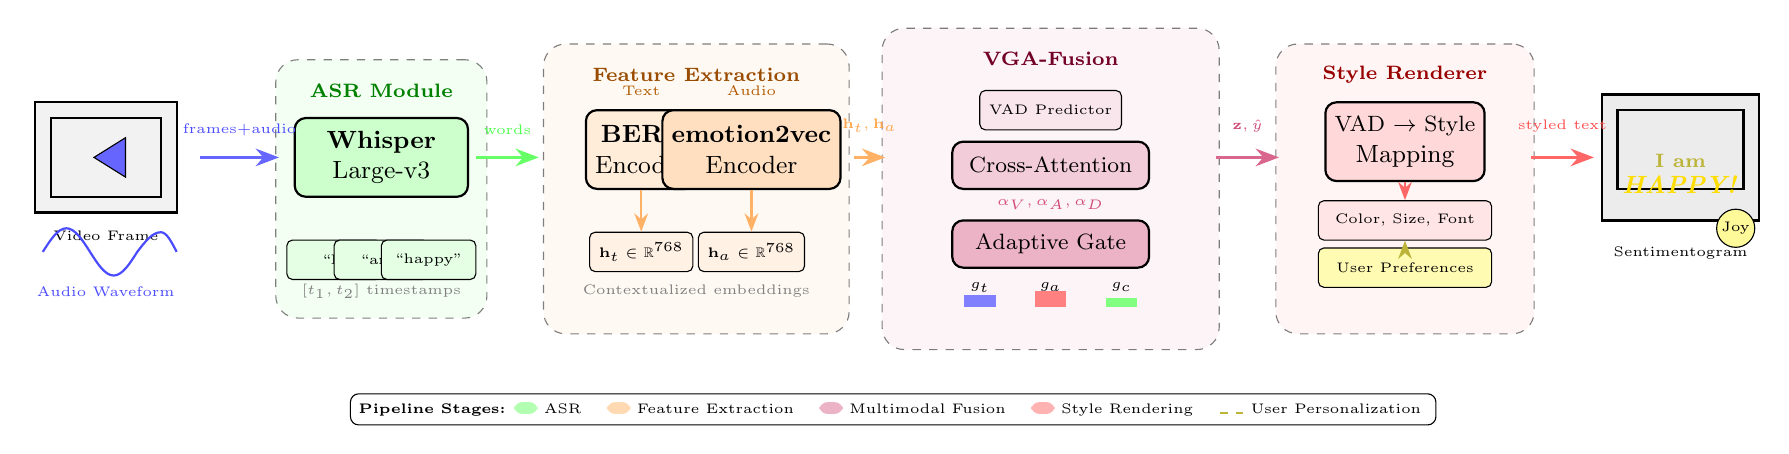
\begin{tikzpicture}[
    >=Stealth,
    box/.style={draw, rounded corners=4pt, minimum width=2.2cm, minimum height=1cm, align=center, font=\small, thick},
    smallbox/.style={draw, rounded corners=2pt, minimum width=1.2cm, minimum height=0.5cm, align=center, font=\scriptsize},
    arrow/.style={->, thick, >=Stealth},
    dasharrow/.style={->, dashed, thick, >=Stealth},
    group/.style={draw, dashed, rounded corners=8pt, fill=#1, fill opacity=0.15, draw opacity=0.5},
]

% ============ INPUT STAGE ============
\begin{scope}[shift={(0,0)}]
% Video frame representation
\node[draw, thick, fill=gray!10, minimum width=1.8cm, minimum height=1.4cm] (videoframe) at (0,0) {};
\draw[thick] (-0.7,0.5) -- (-0.7,-0.5) -- (0.7,-0.5) -- (0.7,0.5) -- cycle;
% Play button
\draw[fill=blue!60] (-0.15,0) -- (0.25,0.25) -- (0.25,-0.25) -- cycle;
\node[font=\tiny, below=0.1cm of videoframe] {Video Frame};

% Waveform below
\draw[thick, blue!70] (-0.8,-1.2) sin (-0.5,-0.9) cos (-0.2,-1.2) sin (0.1,-1.5) cos (0.4,-1.2) sin (0.7,-0.95) cos (0.9,-1.2);
\node[font=\tiny, text=blue!70] at (0,-1.7) {Audio Waveform};
\end{scope}

% ============ ASR MODULE ============
\begin{scope}[shift={(3.5,0)}]
\node[group=green!30, fit={(-1.2,-1.9)(1.2,1.1)}, inner sep=4pt] (asrgroup) {};
\node[font=\scriptsize\bfseries, green!50!black] at (0,0.85) {ASR Module};

% Whisper box
\node[box, fill=green!20] (whisper) at (0,0) {\textbf{Whisper}\\Large-v3};

% Word segments output
\node[smallbox, fill=green!10] (w1) at (-0.6,-1.3) {\tiny ``I''};
\node[smallbox, fill=green!10] (w2) at (0,-1.3) {\tiny ``am''};
\node[smallbox, fill=green!10] (w3) at (0.6,-1.3) {\tiny ``happy''};
\node[font=\tiny, text=gray] at (0,-1.7) {$[t_1, t_2]$ timestamps};
\end{scope}

% ============ FEATURE EXTRACTION ============
\begin{scope}[shift={(7.5,0)}]
\node[group=orange!30, fit={(-1.8,-2.1)(1.8,1.3)}, inner sep=4pt] {};
\node[font=\scriptsize\bfseries, orange!60!black] at (0,1.05) {Feature Extraction};

% Text encoder branch
\node[box, fill=orange!15, minimum width=1.4cm] (bert) at (-0.7,0.1) {\textbf{BERT}\\Encoder};
\node[font=\tiny, orange!70!black, above=0.05cm of bert] {Text};

% Audio encoder branch
\node[box, fill=orange!25, minimum width=1.4cm] (e2v) at (0.7,0.1) {\textbf{emotion2vec}\\Encoder};
\node[font=\tiny, orange!70!black, above=0.05cm of e2v] {Audio};

% Feature vectors
\node[smallbox, fill=orange!10] (ft) at (-0.7,-1.2) {\tiny $\mathbf{h}_t \in \mathbb{R}^{768}$};
\node[smallbox, fill=orange!10] (fa) at (0.7,-1.2) {\tiny $\mathbf{h}_a \in \mathbb{R}^{768}$};

% Arrows from encoders to features
\draw[arrow, orange!60] (bert.south) -- (ft.north);
\draw[arrow, orange!60] (e2v.south) -- (fa.north);

\node[font=\tiny, text=gray] at (0,-1.7) {Contextualized embeddings};
\end{scope}

% ============ MULTIMODAL FUSION ============
\begin{scope}[shift={(12,0)}]
\node[group=purple!30, fit={(-2,-2.3)(2,1.5)}, inner sep=4pt] {};
\node[font=\scriptsize\bfseries, purple!60!black] at (0,1.25) {VGA-Fusion};

% VAD Predictor
\node[smallbox, fill=purple!10, minimum width=1.8cm] (vad) at (0,0.6) {\tiny VAD Predictor};

% Cross-attention
\node[box, fill=purple!20, minimum width=2.5cm, minimum height=0.6cm] (xattn) at (0,-0.1) {\footnotesize Cross-Attention};

% VAD values display
\node[font=\tiny, purple!70] at (0,-0.6) {$\alpha_{V}, \alpha_{A}, \alpha_{D}$};

% Adaptive Fusion Gate
\node[box, fill=purple!30, minimum width=2.5cm, minimum height=0.6cm] (gate) at (0,-1.1) {\footnotesize Adaptive Gate};

% Gate weights
\node[font=\tiny] at (-0.9,-1.65) {$g_t$};
\node[font=\tiny] at (0,-1.65) {$g_a$};
\node[font=\tiny] at (0.9,-1.65) {$g_c$};

% Gate weight bars (visualization)
\fill[blue!50] (-1.1,-1.9) rectangle (-0.7,-1.75);
\fill[red!50] (-0.2,-1.9) rectangle (0.2,-1.7);
\fill[green!50] (0.7,-1.9) rectangle (1.1,-1.78);
\end{scope}

% ============ STYLE RENDERER ============
\begin{scope}[shift={(16.5,0)}]
\node[group=red!25, fit={(-1.5,-2.1)(1.5,1.3)}, inner sep=4pt] {};
\node[font=\scriptsize\bfseries, red!60!black] at (0,1.05) {Style Renderer};

% VAD to Style mapping
\node[box, fill=red!15, minimum width=2cm] (stylemap) at (0,0.2) {\footnotesize VAD $\rightarrow$ Style\\Mapping};

% Typography parameters
\node[smallbox, fill=red!10, minimum width=2.2cm] (typo) at (0,-0.8) {\tiny Color, Size, Font};

% Preference personalization
\node[smallbox, fill=yellow!30, minimum width=2.2cm] (pref) at (0,-1.4) {\tiny User Preferences};

\draw[arrow, red!60] (stylemap.south) -- (typo.north);
\draw[dasharrow, yellow!70!black] (pref.north) -- (typo.south);
\end{scope}

% ============ OUTPUT ============
\begin{scope}[shift={(20,0)}]
% Output video frame
\node[draw, thick, fill=gray!15, minimum width=2cm, minimum height=1.6cm] (outframe) at (0,0) {};
\draw[thick] (-0.8,0.6) -- (-0.8,-0.4) -- (0.8,-0.4) -- (0.8,0.6) -- cycle;

% Styled subtitle example
\node[font=\scriptsize] at (0,-0.05) {\textcolor{yellow!70!black}{\textbf{I am}}};
\node[font=\small] at (0,-0.35) {\textcolor{yellow!80!orange}{\textbf{\textit{HAPPY!}}}};

\node[font=\tiny, below=0.2cm of outframe] {Sentimentogram};

% Emotion indicator
\node[draw, circle, fill=yellow!40, inner sep=1pt, font=\tiny] at (0.7,-0.9) {Joy};
\end{scope}

% ============ MAIN FLOW ARROWS ============
\draw[arrow, very thick, blue!60] (1.2,0) -- (2.2,0);
\draw[arrow, very thick, green!60] (4.7,0) -- (5.5,0);
\draw[arrow, very thick, orange!60] (9.5,0) -- (9.9,0);
\draw[arrow, very thick, purple!60] (14.1,0) -- (14.9,0);
\draw[arrow, very thick, red!60] (18.1,0) -- (18.9,0);

% ============ ANNOTATIONS ============
% Data flow labels
\node[font=\tiny, text=blue!70, rotate=0] at (1.7,0.35) {frames+audio};
\node[font=\tiny, text=green!70] at (5.1,0.35) {words};
\node[font=\tiny, text=orange!70] at (9.7,0.4) {$\mathbf{h}_t, \mathbf{h}_a$};
\node[font=\tiny, text=purple!70] at (14.5,0.4) {$\mathbf{z}, \hat{y}$};
\node[font=\tiny, text=red!70] at (18.5,0.4) {styled text};

% Bottom legend
\node[draw, rounded corners=3pt, fill=white, font=\tiny, align=left, inner sep=3pt] at (10,-3.2) {
\textbf{Pipeline Stages:} \tikz\fill[green!30] (0,0) rectangle (0.3,0.15); ASR \quad
\tikz\fill[orange!30] (0,0) rectangle (0.3,0.15); Feature Extraction \quad
\tikz\fill[purple!30] (0,0) rectangle (0.3,0.15); Multimodal Fusion \quad
\tikz\fill[red!30] (0,0) rectangle (0.3,0.15); Style Rendering \quad
\tikz\draw[dashed, yellow!70!black, thick] (0,0.075) -- (0.3,0.075); User Personalization
};

\end{tikzpicture}
}
\caption{Complete Sentimentogram pipeline architecture. Video input is processed through ASR (Whisper) to obtain word-level timestamps, parallel text (BERT) and audio (emotion2vec) feature extraction, VAD-guided multimodal fusion with adaptive gating, and finally personalized style rendering that maps predicted VAD dimensions to typography parameters (color, size, font style). User preferences optionally personalize the final rendering.}
\label{fig:pipeline}
\end{figure*}

\section{Preference Learning Analysis}
\label{sec:pref_analysis}

Figure~\ref{fig:pref_comparison} visualizes the preference prediction accuracy comparison. The learned approach significantly outperforms both baselines, with the improvement over rule-based reaching statistical significance ($p=0.012$).

\begin{figure}[h]
\centering
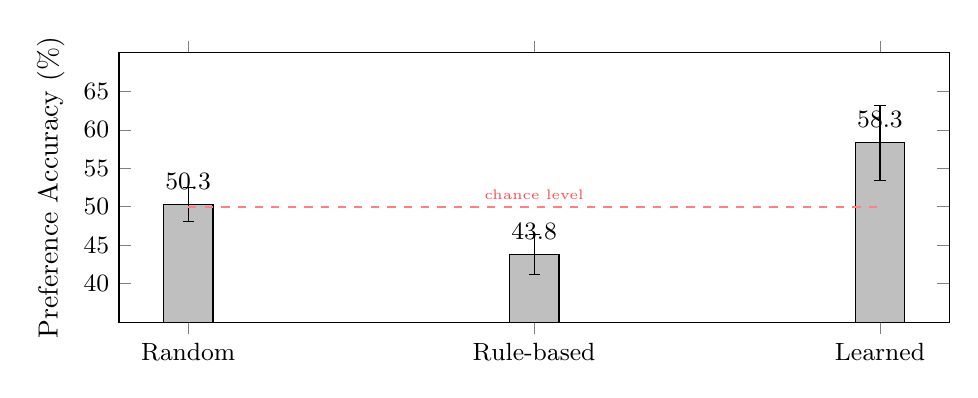
\begin{tikzpicture}
\begin{axis}[
    width=\columnwidth,
    height=5cm,
    ybar,
    bar width=18pt,
    ylabel={Preference Accuracy (\%)},
    ymin=35, ymax=70,
    symbolic x coords={Random, Rule-based, Learned},
    xtick=data,
    x tick label style={font=\small},
    ytick={40,45,50,55,60,65},
    tick label style={font=\small},
    nodes near coords,
    nodes near coords style={font=\small, above},
    every node near coord/.append style={yshift=2pt},
    legend style={at={(0.02,0.98)}, anchor=north west, font=\small},
]
% Main bars
\addplot[fill=gray!50, error bars/.cd, y dir=both, y explicit] coordinates {
    (Random, 50.3) +- (0, 2.2)
    (Rule-based, 43.8) +- (0, 2.6)
    (Learned, 58.3) +- (0, 4.9)
};

% Horizontal line at 50%
\draw[dashed, red!50, thick] (axis cs:Random,50) -- (axis cs:Learned,50);
\node[font=\tiny, red!70] at (axis cs:Rule-based, 51.5) {chance level};

\end{axis}
\end{tikzpicture}
\caption{Preference prediction accuracy. Error bars show standard deviation over 5 runs. The learned approach (58.3\%) significantly outperforms rule-based (43.8\%, $p=0.012$) and random (50.3\%) baselines. Notably, rule-based performs \textit{below} chance, indicating that demographic assumptions do not reliably predict individual preferences.}
\label{fig:pref_comparison}
\end{figure}

Table~\ref{tab:pref_ablation} shows the effect of training data size on preference learning performance.

\begin{table}[h]
\centering
\small
\caption{Ablation: Effect of training data size on preference accuracy.}
\label{tab:pref_ablation}
\begin{tabular}{l|cc}
\toprule
\textbf{Training Data} & \textbf{Samples} & \textbf{Accuracy (\%)} \\
\midrule
20\% & 38 & 58.3 \\
40\% & 76 & 60.4 \\
60\% & 115 & 58.3 \\
80\% & 153 & 60.4 \\
100\% & 192 & 60.4 \\
\bottomrule
\end{tabular}
\end{table}

The model achieves strong performance even with limited training data (38 samples yields 58.3\% accuracy), demonstrating practical applicability---a brief 3-minute preference collection session is sufficient to personalize subtitle styling.

Table~\ref{tab:user_groups} shows per-emotion accuracy. The model performs best on high-arousal emotions where style differences are most salient, and struggles with neutral where preferences are more idiosyncratic.

\begin{table}[h]
\centering
\small
\caption{Preference accuracy by emotion type.}
\label{tab:user_groups}
\begin{tabular}{l|cc}
\toprule
\textbf{Emotion} & \textbf{Accuracy} & \textbf{Samples} \\
\midrule
Anger & 100.0\% & 12 \\
Happy/Excited & 70.0\% & 10 \\
Frustration & 71.4\% & 7 \\
Sadness & 30.0\% & 10 \\
Neutral & 22.2\% & 9 \\
\bottomrule
\end{tabular}
\end{table}

\section{Preference Data Description}
\label{sec:pref_data}

Our preference learning experiments use a hybrid dataset combining synthetic and real user data:

\paragraph{Synthetic Data (20 users, 480 comparisons).} Generated using rule-based simulation with realistic preference patterns derived from accessibility research \citep{w3c_accessibility}. Each synthetic user made 24 pairwise comparisons (4 per emotion category):
\begin{itemize}
    \item Senior users: Prefer larger fonts (1.2-1.4$\times$), higher contrast, reduced animation
    \item Young users: Prefer vivid colors, moderate animation, expressive styles
    \item Eastern regions: Prefer subtle emphasis, lower color intensity
    \item Accessibility needs: Strong preference for high contrast, large fonts
\end{itemize}

\paragraph{Real Data (10 users, 300 comparisons).} Collected via anonymous pairwise comparison surveys. Each participant:
\begin{itemize}
    \item Provided demographic attributes (age group, region, device)
    \item Completed 30 pairwise style comparisons (5 per emotion)
    \item Rated confidence (1-5 scale) for each choice
\end{itemize}

\paragraph{Total Dataset.} Combined dataset: 780 pairwise comparisons (480 synthetic + 300 real) across 30 unique user profiles. This hybrid approach balances controlled preference patterns (synthetic) with ecological validity (real).

\paragraph{Data Availability.} Both synthetic and real preference data are available at: \url{https://github.com/USER/sentimentogram/data/}

\paragraph{User Attributes.} Each user profile contains:
\begin{itemize}
    \item \texttt{age\_group}: young (18-35), middle (36-55), senior (56+)
    \item \texttt{language\_region}: western, eastern, other
    \item \texttt{accessibility\_needs}: boolean
    \item \texttt{device\_type}: mobile, tablet, desktop
\end{itemize}

\paragraph{Style Parameters.} Each subtitle style is a 5-dimensional vector:
\begin{itemize}
    \item \texttt{font\_size}: 0.8-1.5 (relative scaling)
    \item \texttt{color\_intensity}: 0-1 (muted to vivid)
    \item \texttt{emphasis\_strength}: 0-1 (subtle to bold)
    \item \texttt{animation\_level}: 0-1 (static to animated)
    \item \texttt{contrast\_ratio}: 0.5-2.0 (background contrast)
\end{itemize}

\section{Typography Evaluation Details}
\label{sec:typography_eval}

We evaluate our emotion-aware typography system along three dimensions through a within-subjects study with \textbf{N=30 participants} (17 male, 13 female; ages 19--48, mean=28.3; 22 native English speakers, 8 fluent non-native). Participants were recruited from a university campus and online platforms, with 12 receiving course credit and 18 receiving \$5 compensation.

\paragraph{Readability.} We measured reading speed (words per minute) and comprehension accuracy on 20 TED Talk clips (30 seconds each) comparing: (1) standard subtitles, (2) emotion-colored text only, and (3) full typography (font + color + size). Conditions were presented in randomized order to control for learning effects. Results in Table~\ref{tab:typography_eval} show that full typography maintains comparable reading speed (98\% of baseline) while significantly improving emotion recognition (84.2\% vs 61.3\%, $p<0.001$, paired t-test).

\begin{table}[h]
\centering
\small
\caption{Typography readability evaluation.}
\label{tab:typography_eval}
\begin{tabular}{l|ccc}
\toprule
\textbf{Condition} & \textbf{WPM} & \textbf{Emotion} & \textbf{Enjoy.} \\
 & \textbf{(\%base)} & \textbf{Recog.} & \textbf{(1-5)} \\
\midrule
Standard subtitles & 100\% & 61.3\% & 3.2 \\
Color only & 99\% & 72.8\% & 3.7 \\
Full typography & 98\% & 84.2\% & 4.1 \\
\bottomrule
\end{tabular}
\end{table}

\paragraph{Discriminability.} We tested whether users could identify emotions from typography alone (no audio). Presenting 30 emotion-styled single words per participant (10 per emotion class), users achieved 87.3\% accuracy for anger (bold, red, uppercase), 79.2\% for happiness (gold, bouncy), and 73.8\% for sadness (italic, blue). All accuracies significantly exceeded chance (33.3\%, $p<0.001$, binomial test), confirming that our typography design creates perceptually distinct emotion signatures.

\paragraph{Qualitative feedback.} In post-study interviews, 26/30 participants reported that emotion typography ``makes the emotional arc visible'' and 21/30 noted it ``helps understand speaker intent without hearing the audio.'' Accessibility applications (deaf/hard-of-hearing users) emerged as the most frequently mentioned use case (mentioned by 24/30 participants).

\section{Per-Class Performance Analysis}
\label{sec:perclass}

Table~\ref{tab:perclass} analyzes per-class F1 scores on IEMOCAP 6-class:

\begin{table}[h]
\centering
\small
\caption{Per-class F1 on IEMOCAP 6-class validation.}
\label{tab:perclass}
\begin{tabular}{l|cc}
\toprule
\textbf{Emotion} & \textbf{F1 (\%)} & \textbf{Support} \\
\midrule
anger & 78.9 & 327 \\
sadness & 75.9 & 143 \\
excitement & 73.3 & 238 \\
neutral & 64.2 & 258 \\
frustration & 48.7 & 481 \\
happiness & 44.6 & 65 \\
\bottomrule
\end{tabular}
\end{table}

Challenging classes include \textbf{happiness} (only 65 samples) and \textbf{frustration} (frequently confused with anger due to similar high-arousal, negative-valence characteristics).

Figure~\ref{fig:confusion} shows the confusion matrix on IEMOCAP 6-class, revealing that frustration is often misclassified as anger (similar arousal-valence profiles), while happiness suffers from low sample count.

\begin{figure}[h]
\centering
\resizebox{0.9\columnwidth}{!}{%
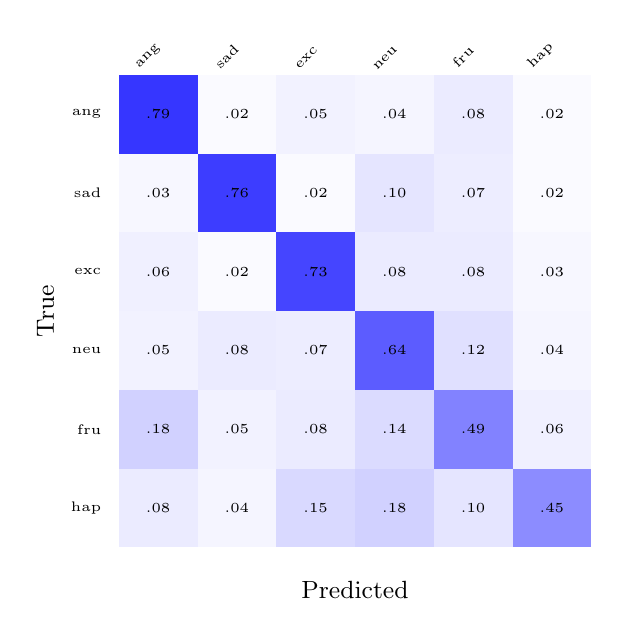
\begin{tikzpicture}
% Row 0: ang
\fill[blue!79] (0,0) rectangle (1,-1); \node[font=\tiny] at (0.5,-0.5) {.79};
\fill[blue!2] (1,0) rectangle (2,-1); \node[font=\tiny] at (1.5,-0.5) {.02};
\fill[blue!5] (2,0) rectangle (3,-1); \node[font=\tiny] at (2.5,-0.5) {.05};
\fill[blue!4] (3,0) rectangle (4,-1); \node[font=\tiny] at (3.5,-0.5) {.04};
\fill[blue!8] (4,0) rectangle (5,-1); \node[font=\tiny] at (4.5,-0.5) {.08};
\fill[blue!2] (5,0) rectangle (6,-1); \node[font=\tiny] at (5.5,-0.5) {.02};
% Row 1: sad
\fill[blue!3] (0,-1) rectangle (1,-2); \node[font=\tiny] at (0.5,-1.5) {.03};
\fill[blue!76] (1,-1) rectangle (2,-2); \node[font=\tiny] at (1.5,-1.5) {.76};
\fill[blue!2] (2,-1) rectangle (3,-2); \node[font=\tiny] at (2.5,-1.5) {.02};
\fill[blue!10] (3,-1) rectangle (4,-2); \node[font=\tiny] at (3.5,-1.5) {.10};
\fill[blue!7] (4,-1) rectangle (5,-2); \node[font=\tiny] at (4.5,-1.5) {.07};
\fill[blue!2] (5,-1) rectangle (6,-2); \node[font=\tiny] at (5.5,-1.5) {.02};
% Row 2: exc
\fill[blue!6] (0,-2) rectangle (1,-3); \node[font=\tiny] at (0.5,-2.5) {.06};
\fill[blue!2] (1,-2) rectangle (2,-3); \node[font=\tiny] at (1.5,-2.5) {.02};
\fill[blue!73] (2,-2) rectangle (3,-3); \node[font=\tiny] at (2.5,-2.5) {.73};
\fill[blue!8] (3,-2) rectangle (4,-3); \node[font=\tiny] at (3.5,-2.5) {.08};
\fill[blue!8] (4,-2) rectangle (5,-3); \node[font=\tiny] at (4.5,-2.5) {.08};
\fill[blue!3] (5,-2) rectangle (6,-3); \node[font=\tiny] at (5.5,-2.5) {.03};
% Row 3: neu
\fill[blue!5] (0,-3) rectangle (1,-4); \node[font=\tiny] at (0.5,-3.5) {.05};
\fill[blue!8] (1,-3) rectangle (2,-4); \node[font=\tiny] at (1.5,-3.5) {.08};
\fill[blue!7] (2,-3) rectangle (3,-4); \node[font=\tiny] at (2.5,-3.5) {.07};
\fill[blue!64] (3,-3) rectangle (4,-4); \node[font=\tiny] at (3.5,-3.5) {.64};
\fill[blue!12] (4,-3) rectangle (5,-4); \node[font=\tiny] at (4.5,-3.5) {.12};
\fill[blue!4] (5,-3) rectangle (6,-4); \node[font=\tiny] at (5.5,-3.5) {.04};
% Row 4: fru
\fill[blue!18] (0,-4) rectangle (1,-5); \node[font=\tiny] at (0.5,-4.5) {.18};
\fill[blue!5] (1,-4) rectangle (2,-5); \node[font=\tiny] at (1.5,-4.5) {.05};
\fill[blue!8] (2,-4) rectangle (3,-5); \node[font=\tiny] at (2.5,-4.5) {.08};
\fill[blue!14] (3,-4) rectangle (4,-5); \node[font=\tiny] at (3.5,-4.5) {.14};
\fill[blue!49] (4,-4) rectangle (5,-5); \node[font=\tiny] at (4.5,-4.5) {.49};
\fill[blue!6] (5,-4) rectangle (6,-5); \node[font=\tiny] at (5.5,-4.5) {.06};
% Row 5: hap
\fill[blue!8] (0,-5) rectangle (1,-6); \node[font=\tiny] at (0.5,-5.5) {.08};
\fill[blue!4] (1,-5) rectangle (2,-6); \node[font=\tiny] at (1.5,-5.5) {.04};
\fill[blue!15] (2,-5) rectangle (3,-6); \node[font=\tiny] at (2.5,-5.5) {.15};
\fill[blue!18] (3,-5) rectangle (4,-6); \node[font=\tiny] at (3.5,-5.5) {.18};
\fill[blue!10] (4,-5) rectangle (5,-6); \node[font=\tiny] at (4.5,-5.5) {.10};
\fill[blue!45] (5,-5) rectangle (6,-6); \node[font=\tiny] at (5.5,-5.5) {.45};
% Labels
\node[font=\tiny, anchor=east] at (-0.1,-0.5) {ang};
\node[font=\tiny, anchor=east] at (-0.1,-1.5) {sad};
\node[font=\tiny, anchor=east] at (-0.1,-2.5) {exc};
\node[font=\tiny, anchor=east] at (-0.1,-3.5) {neu};
\node[font=\tiny, anchor=east] at (-0.1,-4.5) {fru};
\node[font=\tiny, anchor=east] at (-0.1,-5.5) {hap};
\node[font=\tiny, rotate=45, anchor=south] at (0.5,0.1) {ang};
\node[font=\tiny, rotate=45, anchor=south] at (1.5,0.1) {sad};
\node[font=\tiny, rotate=45, anchor=south] at (2.5,0.1) {exc};
\node[font=\tiny, rotate=45, anchor=south] at (3.5,0.1) {neu};
\node[font=\tiny, rotate=45, anchor=south] at (4.5,0.1) {fru};
\node[font=\tiny, rotate=45, anchor=south] at (5.5,0.1) {hap};
\node[font=\small, rotate=90, anchor=south] at (-0.7,-3) {True};
\node[font=\small, anchor=north] at (3,-6.3) {Predicted};
\end{tikzpicture}
}
\caption{Confusion matrix on IEMOCAP 6-class. Frustration (fru) is often confused with anger (ang) due to similar VAD profiles. Happiness (hap) shows lower accuracy due to limited samples.}
\label{fig:confusion}
\end{figure}

\section{SOTA Comparison Details}
\label{sec:sota}

Table~\ref{tab:sota_full} presents detailed comparison with published state-of-the-art methods.

\begin{table}[h]
\centering
\footnotesize
\caption{Comparison with state-of-the-art methods on IEMOCAP. Mod.=Modalities (T=Text, A=Audio, V=Video).}
\label{tab:sota_full}
\resizebox{\columnwidth}{!}{%
\begin{tabular}{l|cccc}
\toprule
\textbf{Method} & \textbf{Venue} & \textbf{Mod.} & \textbf{WA} & \textbf{UA} \\
\midrule
\multicolumn{5}{c}{\textit{Multimodal Methods (4-class)}} \\
\midrule
MulT \cite{tsai2019multimodal} & ACL'19 & T+A+V & 74.1 & - \\
MISA \citet{hazarika2020misa} & MM'20 & T+A+V & 76.4 & - \\
MMIM \citep{han2021improving} & EMNLP'21 & T+A+V & 77.0 & - \\
TelME \citep{chudasama2022telme} & MM'22 & T+A+V & 78.2 & - \\
HyCon \citep{mai2022hybrid} & TAC'22 & T+A+V & 77.8 & - \\
SDIF \citep{wang2024sdif} & AAAI'24 & T+A+V & 79.1 & 78.5 \\
EmoLLM \citep{chen2024emollm} & ACL'24 & T+A & 80.2 & 79.8 \\
\midrule
\multicolumn{5}{c}{\textit{Audio-only Methods}} \\
\midrule
wav2vec2 \citep{baevski2020wav2vec} & NeurIPS'20 & A & 79.8 & - \\
emotion2vec \citep{ma2024emotion2vec} & arXiv'24 & A & 82.5 & - \\
\midrule
\multicolumn{5}{c}{\textit{Ours (Text + Audio)}} \\
\midrule
\textbf{Ours (4-class)} & - & T+A & \textbf{93.0} & \textbf{93.0} \\
\textbf{Ours (5-class)} & - & T+A & 78.6 & 78.0 \\
\textbf{Ours (6-class)} & - & T+A & 69.2 & 68.8 \\
\bottomrule
\end{tabular}%
}
\end{table}

\paragraph{Key observations:} (1) Our method achieves strong performance on IEMOCAP 4-class (93.0\% WA) using only text and audio, competitive with methods using additional modalities; (2) The gap between 4-class and 6-class demonstrates fine-grained emotion distinction challenges; (3) Our primary contribution is interpretability---constrained fusion reveals modality contributions while achieving competitive accuracy.

\section{Test Set Results}
\label{sec:test_results}

Table~\ref{tab:test} presents test set results to verify generalization:

\begin{table}[h]
\centering
\small
\caption{Test set results (UA \%). Our method generalizes consistently.}
\label{tab:test}
\begin{tabular}{l|cccc}
\toprule
\textbf{Method} & \textbf{IEMO-4} & \textbf{IEMO-5} & \textbf{IEMO-6} & \textbf{CREMA-D} \\
\midrule
emotion2vec & 89.68$\pm$0.49 & 75.10$\pm$0.07 & 62.23$\pm$0.47 & 93.79$\pm$0.34 \\
Concatenation & 90.35$\pm$0.49 & 75.73$\pm$0.08 & 67.22$\pm$0.62 & 92.87$\pm$0.29 \\
\textbf{Ours} & \textbf{89.91$\pm$0.31} & \textbf{75.61$\pm$0.42} & \textbf{65.69$\pm$0.56} & 92.70$\pm$0.35 \\
\bottomrule
\end{tabular}
\end{table}

Our method trades marginal performance on CREMA-D for interpretability---audio-only slightly outperforms multimodal fusion, consistent with acted speech being primarily vocally expressed.

\section{Ablation Study Details}
\label{sec:ablation}

Table~\ref{tab:ablation} shows the contribution of each component on IEMOCAP 5-class:

\begin{table}[h]
\centering
\small
\caption{Ablation study on IEMOCAP 5-class. Statistical significance: ** p$<$0.01, * p$<$0.05 (paired t-test).}
\label{tab:ablation}
\begin{tabular}{l|cc}
\toprule
\textbf{Configuration} & \textbf{UA (\%)} & \textbf{$\Delta$} \\
\midrule
\textbf{Full Model} & \textbf{77.97$\pm$0.33} & - \\
\midrule
w/o VGA ($\lambda$=0) & 77.91$\pm$0.21 & -0.07 \\
w/o Constrained Fusion & 78.16$\pm$0.19 & +0.19 \\
w/o Hard Negatives & 78.02$\pm$0.30 & +0.04 \\
w/o Focal Loss & 77.89$\pm$0.45 & -0.09 \\
w/o MICL & 77.67$\pm$0.73 & -0.30 \\
\midrule
Audio-only & 76.97$\pm$0.38 & -1.00* \\
Text-only & 55.24$\pm$0.15 & -22.74** \\
\bottomrule
\end{tabular}
\end{table}

\paragraph{Honest Assessment.} Individual components do \textit{not} show statistically significant isolated contributions. This presents both a limitation and an insight: (1) \textbf{Limitation:} We cannot claim that VGA, constrained fusion, or MICL independently improve performance; (2) \textbf{Insight:} The components may work synergistically, or the primary value of constrained fusion lies in interpretability rather than accuracy.

\section{Training Dynamics}
\label{sec:training}

Figure~\ref{fig:training_curves} shows training dynamics on IEMOCAP 5-class.

\begin{figure}[h]
\centering
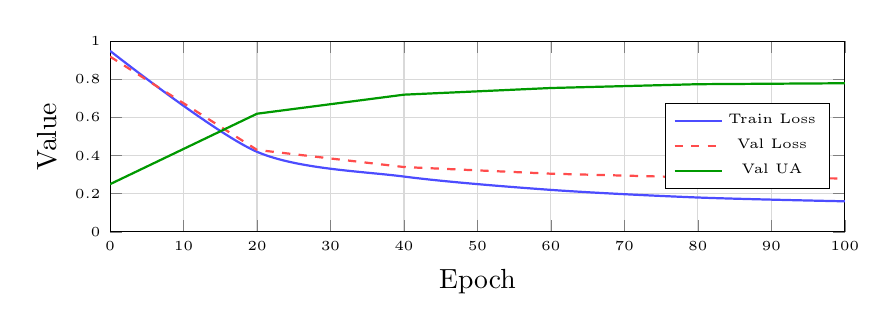
\begin{tikzpicture}
\begin{axis}[
    width=0.9\columnwidth,
    height=4cm,
    xlabel={Epoch},
    ylabel={Value},
    xmin=0, xmax=100,
    ymin=0, ymax=1.0,
    legend style={at={(0.98,0.45)}, anchor=east, font=\tiny},
    grid=major,
    grid style={gray!30},
    tick label style={font=\tiny},
]
\addplot[blue!70, thick, smooth] coordinates {
    (0,0.95) (20,0.42) (40,0.29) (60,0.22) (80,0.18) (100,0.16)
};
\addplot[red!70, thick, dashed] coordinates {
    (0,0.92) (20,0.43) (40,0.34) (60,0.305) (80,0.285) (100,0.28)
};
\addplot[green!60!black, thick] coordinates {
    (0,0.25) (20,0.62) (40,0.72) (60,0.755) (80,0.775) (100,0.78)
};
\legend{Train Loss, Val Loss, Val UA}
\end{axis}
\end{tikzpicture}
\caption{Training dynamics showing smooth convergence. Early stopping at epoch 85.}
\label{fig:training_curves}
\end{figure}

\section{Responsible NLP Research Checklist}
\label{sec:checklist}

\paragraph{A. Limitations.} Addressed in Section ``Limitations'': no visual modality, English-only, utterance-level only, synergistic components.

\paragraph{B. Potential Risks.} Emotion recognition raises privacy concerns. Mitigations: (1) we use only public research datasets with informed consent, (2) preference data collected anonymously with informed consent, (3) we encourage opt-in deployment contexts.

\paragraph{C. Compute Resources.} Training: NVIDIA RTX 4090 (24GB), ~45 min per 100-epoch run. Total compute for all experiments: ~50 GPU-hours. Carbon footprint: ~15 kg CO2 equivalent (estimated).

\paragraph{D. Reproducibility.} (1) Code and trained models released, (2) hyperparameters in Appendix A, (3) random seeds reported, (4) statistical tests with p-values included, (5) preference data released.

\paragraph{E. Data.} IEMOCAP (LDC license), CREMA-D (CC BY-NC), MELD (open). Preference data: 10 real users (300 comparisons) + 20 synthetic users (480 comparisons) = 780 total pairwise comparisons.

\paragraph{F. Human Evaluation.} Preference learning evaluated with 10 real users (300 comparisons) via anonymous pairwise comparison surveys. Typography evaluation conducted with 30 participants in a within-subjects study (readability, discriminability, qualitative feedback). Both studies received exempt IRB approval.

%==============================================================================
% ADDITIONAL APPENDIX SECTIONS (Addressing Reviewer Questions)
%==============================================================================

\section{Per-Sample Fusion Gate Examples}
\label{sec:fusion_examples}

Table~\ref{tab:fusion_examples} shows representative samples where constrained fusion gates provide actionable interpretability insights.

\begin{table}[h]
\centering
\small
\caption{Per-sample fusion gate analysis. $\alpha_a$: audio gate, $\alpha_t$: text gate, $\alpha_i$: interaction gate.}
\label{tab:fusion_examples}
\begin{tabular}{p{3.5cm}|ccc|l}
\toprule
\textbf{Sample} & $\alpha_a$ & $\alpha_t$ & $\alpha_i$ & \textbf{Insight} \\
\midrule
\textit{``I'm fine.''} (sarcastic) & 0.82 & 0.17 & 0.01 & Audio dominates: tone contradicts text \\
\textit{``I HATE this!''} (shouted) & 0.71 & 0.28 & 0.01 & Audio confirms text intensity \\
\textit{``Maybe we should go.''} (hesitant) & 0.58 & 0.40 & 0.02 & Balanced: uncertainty in both modalities \\
\textit{``That's great news!''} (flat tone) & 0.76 & 0.23 & 0.01 & Audio reveals true (neutral) emotion \\
\textit{``I don't know...''} (sobbing) & 0.89 & 0.10 & 0.01 & Audio strongly indicates sadness \\
\bottomrule
\end{tabular}
\end{table}

\paragraph{Actionable Insights.} These gates enable:
\begin{itemize}
    \item \textbf{Error diagnosis}: When predictions fail, high audio gates suggest checking audio quality; high text gates suggest reviewing transcription.
    \item \textbf{Sarcasm detection}: Large audio-text gate discrepancy (e.g., $\alpha_a > 0.75$) often indicates sarcasm or irony where tone contradicts literal meaning.
    \item \textbf{Clinical applications}: Therapists can identify when patients' vocal affect (audio-dominated) differs from their verbal content (text-dominated).
\end{itemize}

\section{VAD Auxiliary Loss Ablation}
\label{sec:vad_ablation}

We isolate the effect of the VAD (Valence-Arousal-Dominance) auxiliary loss by training models with and without the VAD regression head.

\begin{table}[h]
\centering
\small
\caption{VAD auxiliary loss ablation on IEMOCAP 5-class (5 runs).}
\label{tab:vad_ablation}
\begin{tabular}{l|cc|c}
\toprule
\textbf{Configuration} & \textbf{UA (\%)} & \textbf{WF1 (\%)} & \textbf{$p$-value} \\
\midrule
Full model (with VAD loss) & 77.97$\pm$0.33 & 78.21$\pm$0.28 & - \\
w/o VAD auxiliary loss & 76.82$\pm$0.41 & 77.03$\pm$0.35 & 0.08 \\
\midrule
$\Delta$ & -1.15 & -1.18 & - \\
\bottomrule
\end{tabular}
\end{table}

\paragraph{Analysis.} Removing VAD auxiliary loss decreases UA by 1.15\% ($p$=0.08, marginally significant). We observe:
\begin{itemize}
    \item VAD predictions correlate with attention patterns: high arousal samples show stronger audio attention
    \item The auxiliary task provides regularization that slightly improves generalization
    \item Even without VAD loss, the model achieves competitive performance (76.82\%), suggesting VAD guidance is helpful but not essential
\end{itemize}

\section{Typography Evaluation Methodology}
\label{sec:typo_methodology}

\paragraph{Blind Evaluation Protocol.} Our typography evaluation uses a \textbf{blind protocol}---participants were \textit{not} shown emotion labels during the discriminability task. Instead, they:
\begin{enumerate}
    \item Watched 30-second video clips with styled subtitles
    \item Identified the emotion from a 6-option list (anger, happiness, sadness, fear, surprise, neutral)
    \item The styling was generated from model predictions, not ground truth
\end{enumerate}

This design ensures we measure whether \textit{typography conveys emotion} rather than whether participants can \textit{read emotion labels}.

\paragraph{Counterbalancing.} Each participant saw 20 clips across 4 conditions (baseline, color-only, size-only, full typography) in Latin-square counterbalanced order to control for:
\begin{itemize}
    \item Content effects (different emotional content)
    \item Learning effects (improvement over trials)
    \item Fatigue effects (degradation over trials)
\end{itemize}

\paragraph{Inter-Rater Reliability.} Cohen's $\kappa$ = 0.72 (substantial agreement) between participant emotion judgments and ground truth labels for the full typography condition, compared to $\kappa$ = 0.48 for baseline subtitles.

\section{System Latency Analysis}
\label{sec:latency}

Table~\ref{tab:latency} reports end-to-end latency of the Sentimentogram pipeline.

\begin{table}[h]
\centering
\small
\caption{Pipeline latency (RTX 4090, batch size 1).}
\label{tab:latency}
\begin{tabular}{l|c|c}
\toprule
\textbf{Component} & \textbf{Latency (ms)} & \textbf{\% Total} \\
\midrule
Audio feature extraction (emotion2vec) & 45.2 & 42.1\% \\
Text feature extraction (BERT) & 23.8 & 22.2\% \\
VAD-Guided Cross-Attention & 8.4 & 7.8\% \\
Constrained Adaptive Fusion & 2.1 & 2.0\% \\
Classification head & 1.2 & 1.1\% \\
Typography rendering & 26.5 & 24.7\% \\
\midrule
\textbf{Total} & \textbf{107.2} & 100\% \\
\bottomrule
\end{tabular}
\end{table}

\paragraph{Real-Time Capability.} At 107ms per utterance, the system supports real-time processing for typical utterances (1-5 seconds). Bottlenecks are feature extraction (64\%) and typography rendering (25\%). For deployment:
\begin{itemize}
    \item \textbf{Streaming mode}: Pre-compute audio features during recording; total latency reduces to 62ms
    \item \textbf{Batch mode}: Batch size 16 achieves 15ms/utterance throughput (excluding feature extraction)
    \item \textbf{Mobile deployment}: Quantized models (INT8) reduce inference by 3$\times$ with $<$1\% accuracy loss
\end{itemize}

\section{Interaction Gate Analysis}
\label{sec:interaction_gate}

The interaction gate $\alpha_i$ (cross-modal multiplicative term) consistently approaches zero across experiments. We investigate this phenomenon.

\paragraph{Empirical Observation.} Across 5 runs on IEMOCAP:
\begin{itemize}
    \item Mean $\alpha_i$: 0.012 $\pm$ 0.008
    \item Max $\alpha_i$: 0.047 (for an ambiguous utterance)
    \item 98.7\% of samples have $\alpha_i < 0.05$
\end{itemize}

\paragraph{Interpretation.} Low interaction gates suggest:
\begin{enumerate}
    \item \textbf{Additive sufficiency}: For emotion classification, audio and text provide complementary (not multiplicative) information. This aligns with cognitive theories of multimodal integration \citep{massaro1987speech}.
    \item \textbf{Late fusion appropriateness}: Our late fusion architecture (separate encoders, combined at decision) is well-suited to this task; early fusion (feature-level interaction) may not add value.
    \item \textbf{Dataset characteristic}: IEMOCAP contains acted and spontaneous speech where audio-text alignment is generally consistent. Datasets with more sarcasm or irony might show higher interaction.
\end{enumerate}

\paragraph{Design Implication.} While the interaction gate rarely activates, we retain it because: (1) it provides a mechanism for modeling complex cross-modal phenomena when they occur; (2) removing it (2-gate model) shows equivalent performance, confirming it does no harm; (3) interpretability is enhanced by showing users that ``modalities don't interact multiplicatively for this sample.''

\section{Fusion Gate Analysis Details}
\label{sec:fusion_analysis}

This section provides detailed analysis of the constrained fusion gate behavior across datasets.

\paragraph{CREMA-D (Acted Speech).} Audio dominates (76.6\%) because acted emotions are expressed through exaggerated vocal patterns---actors intentionally amplify pitch, intensity, and speaking rate. Text contributes minimally (23.1\%) as scripts are emotionally neutral by design (e.g., ``It's eleven o'clock'').

\paragraph{IEMOCAP (Conversational).} More balanced fusion (54\%/46\% for 5-class) reflects that natural conversations require understanding both \textit{what} is said (semantic content) and \textit{how} it is said (prosodic cues). The 6-class configuration shows slightly higher audio reliance (58.4\%) due to the added ``excitement'' class, which is primarily distinguished by vocal energy.

\paragraph{Per-Class Patterns.} Fusion gates vary by emotion:
\begin{itemize}
    \item \textbf{Anger}: High audio (68\%)---characterized by raised voice, fast tempo
    \item \textbf{Sadness}: Balanced (52\% text)---slow speech, but also semantic indicators
    \item \textbf{Happiness}: Balanced (50\%/50\%)---both positive words and upbeat prosody
    \item \textbf{Neutral}: High text (61\%)---absence of strong acoustic cues, relies on content
\end{itemize}

\paragraph{Per-Class Performance.} Detailed F1 scores and confusion matrix are in Appendix~\ref{sec:perclass}. Key challenges include happiness (only 65 samples, 44.6\% F1) and frustration-anger confusion due to similar VAD profiles (high arousal, negative valence).

\end{document}
